\chapter{Two-source high harmonic generation}
\label{chap:two_source}

\section{Introduction}
\label{sec:intro_ts}

A common difficulty in working with extreme ultraviolet (XUV) light is the lack of efficient and broadband optics, especially beam splitters. In this chapter, I will introduce a method for generating two sources of XUV light by high harmonic generation (HHG) using a square-wave phase grating (SWPG).  This SWPG allows for the duplication of an infrared (IR) pulse, as well as precise and stable control of the relative phase between the duplicates of the input IR pulse. The two most intense duplicates can generate harmonics which will interfere in the far-field. This can be thought of as an inline Mach-Zehnder interferometer with interferometric stability on sub-wavelength level of the high harmonic. The inherent stability of this two-source scheme will be utilized to measure both the real and imaginary parts of the refractive index of a medium.

\section{Theory}
\subsection{Laser beam shaping using diffractive optics}
\label{sec:beam_shaping}
%Describe general problem of beam shaping using DOEs. see \cite{romeroMathematicalAspectsLaser2010,romeroMathematicalTheoryLaser2010,romeroTheoryOptimalBeam2007}
%!!!!!!!!!!!!!!!!!!!!!!!!!!!!!!!!!!!!!!!!!!!!!!!!!!!!!!!!!!!!!!!!!!!!!!!!!!!!!!!!!!!!!!!!!!!!!!!!!!!!!!!!!!!!!!!!!!
%!!!!!!!!!!!!!!!!!!!!!!!!!!!!!!!!!COME BACK TO THIS SECTION LATER!!!!!!!!!!!!!!!!!!!!!!!!!!!!!!!!!!!!!!!!!!!!!!!!!!
%!!!!!!!!!!!!!!!!!!!!!!!!!!!!!!!!!!!!!!!!!!!!!!!!!!!!!!!!!!!!!!!!!!!!!!!!!!!!!!!!!!!!!!!!!!!!!!!!!!!!!!!!!!!!!!!!!!

In many experimental designs, it is advantageous to be able to shape the spatial intensity distribution of light to be something other than a typical Gaussian beam.  A common example of this is generating a beam with an approximately constant intensity across it's spatial profile (a flat-top beam).  For the experiments described herein, we will be interested in duplicating an input beam with relative phase control between the two duplicate beams.  Both of these examples are part of the general concept of laser beam shaping.  The challenge is to design an optical system such that given an input beam profile $I_{in}(x,y)$ we can generate the desired output beam profile $I_{out}(x,y)$. Ideally, this optical system is designed in such a way that it can be nearly lossless.  The relevant optical system which will be discussed in this chapter is shown in figure \ref{fig:beam_shaping_scheme}.  The system consists of a phase element which modifies the phase of the input field by $\phi(x,y)$ and a Fourier transform lens which adds a quadratic phase to the beam to focus it at the focal plane.  By appropriate choice of the phase profile of the phase element, one can produce the desired beam profile at the focal plane.


\begin{figure}
	\centering
	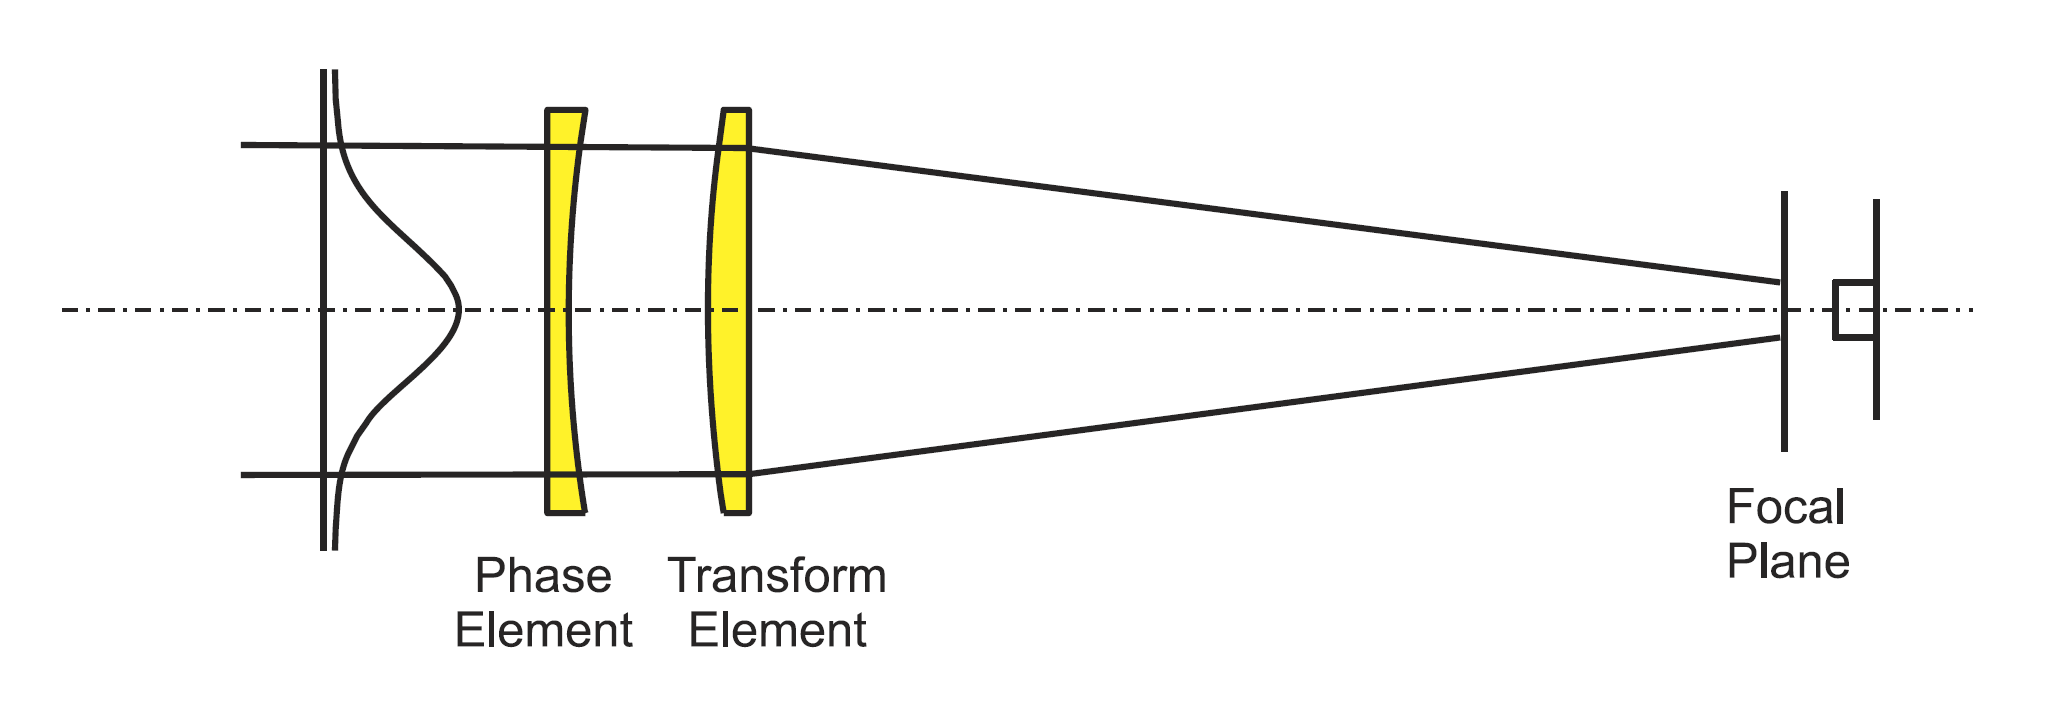
\includegraphics[width=0.9\textwidth]{figures/Two_source/romero_beam_shaping_schematic.png}
	\caption{Schematic demonstrating how to use a diffractive optical element to shape the beam profile at the focal plane. A collimated coherent beam is incident upon a diffractive optical element which shapes the phase of the incident beam, and then a lens is used as a transform element to Fourier transform the beam at the focal plane.  The intensity profile at the focal plane can be controlled by altering the spatial dependence of the phase imparted upon the incident beam by the phase element. Adapted from \cite{romeroMathematicalAspectsLaser2010}}
	\label{fig:beam_shaping_scheme}
\end{figure}


This problem can be theoretically described in terms of Fourier optics \cite{dickeyLaserBeamShaping2000, romeroMathematicalAspectsLaser2010, goodmanIntroductionFourierOptics2005}.  If one assumes that a field $u(x,y,0)$ is incident upon an an aperture at $z=0$, then the field for $z>0$ can be written under the Fresnel approximation by the Fresnel integral
\begin{equation}
\label{fresnel_integral}
	u(x,y,z)=\frac{i k}{2\pi z}e^{i k z}e^{i k (x^2+y^2)/2z}\int_{-\infty}^{\infty}\int_{-\infty}^{\infty}u(\xi,\eta,0) e^{ik(\xi^{2}+\eta^{2})/2z} e^{-ik(x\xi + y\eta)/z} \diff\xi\diff\eta
\end{equation}
where $u(\xi,\eta,0)$ is the incoming field and $k=2\pi/\lambda$ is the wavenumber.  Now, if one assumes that the phase element is placed at $z=0$, then immediately after passing through the thin phase element in Fig. \ref{fig:beam_shaping_scheme} the field is given by
\begin{equation}
	u(\xi,\eta,0)=f(\xi,\eta)e^{i\phi(\xi,\eta)}.
\end{equation} 
After propagating through the thin Fourier transform lens of focal length $f$, a phase of $k(\xi^2\eta^2)/2f$ is added to the beam, and the field at the focal plane is now given by
\begin{equation}
\label{eqn:field_at_focus}
	u(x,y,f)=\frac{ik}{2\pi f}e^{ikf}e^{ik(x^2+y^2)/2f}\int_{-\infty}^{\infty}\int_{-\infty}^{\infty}f(\xi,\eta)e^{i\phi(\xi,\eta)}
	e^{-ik(x\xi + y\eta)/f}\diff\xi\diff\eta
\end{equation}
where the quadratic phase in integral of equation \ref{fresnel_integral} is exactly canceled by the quadratic phase introduced by the lens.

Now, the idea is to rewrite this field profile at the focal plane into a more intuitive form by introducing the equation
\begin{equation}
	g(\xi,\eta)=\frac{ik}{2\pi f}f(\xi,\eta)e^{i\psi(\xi,\eta)}.
\end{equation}
The Fourier transform of this function $g(\xi,\eta)$ is given by
\begin{equation}
\label{eqn:big_G}
	G(a,b)=\frac{ik}{2\pi f}\int_{-\infty}^{\infty}\int_{-\infty}^{\infty}f(\xi,\eta)e^{i\psi(\xi,\eta)}
	e^{-i(a\xi + b\eta)}\diff\xi\diff\eta.
\end{equation}
By setting $a=kx/f$ and $b=ky/f$ and taking the square complex modulus, one obtains the equation
\begin{equation}
	\rvert G(kx/f,ky/f)\rvert^{2} = \frac{k^2}{(2\pi f)^2} \bigg\rvert\int_{-\infty}^{\infty}\int_{-\infty}^{\infty}
	f(\xi,\eta)e^{i\psi(\xi,\eta)}e^{-ik(x\xi+y\eta)/f}\diff\xi\diff\eta\bigg\rvert^{2}.
\end{equation}
By comparing this equation with the square complex modulus of the field at the focal plane (equation \ref{eqn:field_at_focus}), one finds the relationship
\begin{equation}
\label{eqn:Fourier_focal_plane}
	\rvert u(x,y,f)\rvert^2 = \rvert G(kx/f,ky/f)\rvert^2.
\end{equation}

From this last equality we have shown that the intensity of the field at at the focal plane $\rvert u(z=f)\rvert^2$, is given by the Fourier transform of the combined phase imparted upon the incident field by both the phase element and the Fourier transform lens, $\rvert G\rvert^2$. So, if one wants a specific beam shape $Q(x,y)$ at the focal plane, then by tuning the frequency components of the phase imparted upon the beam $\phi(x,y)$ and the focal length $f$ used then one can achieve the desired beam profile, such that
\begin{equation}
\label{eqn:beam_shaping_equality}
	\rvert G(kx/f,ky/f)\rvert^2=Q(x,y).
\end{equation}
This problem is difficult in general, so the challenge in many beam shaping problems is to try and minimize the error between the actual beam profile and the desired profile, and, to further complicate the matter, many applications will require different notions of error to be used.  For example, if one needs the energy distribution to be as close as possible to the desired profile, then the $\ell_2$-norm would be appropriate.  However, if the maximum intensity is of concern, then the $\ell_\infty$-norm combined with the $\ell_2$-norm would be the appropriate notion of error.

It is possible to gain more insight into how difficult a beam shaping problem will be by reformulating the problem in terms of relevant length scales \cite{dickeyLaserBeamShaping2000,romeroMathematicalAspectsLaser2010}.  The idea is to introduce a dimensionless parameter whose magnitude will reflect the validity of underlying assumptions, and so for a given value of this parameter one can intuitively understand the performance (or lack thereof) of the beam shaping system.  This is done by reformulating the above situation in terms of the natural length scales of both the incoming field and the desired field at the focal plane
\begin{align}
	I_{\mathrm{input}} &= \rvert f(x,y)\rvert^2=\rvert\hat{f}(x/\sigma,y/\sigma)\rvert^2\\
	I_{\mathrm{desired}} &= Q(x,y)=\hat{Q}(x/d,y/d)
\end{align}
where $\sigma$ is the characteristic length scale of the input field (typically the beam radius) and $d$ is the characteristic length scale of the desired field.  By expressing the fields in this way, we can now introduce the dimensionless parameter
\begin{equation}
\label{eqn:beta_parameter}
	\beta=\frac{2\pi\sigma D}{\lambda f}.
\end{equation}
Using this dimensionless parameter, one can rewrite equations \ref{eqn:big_G} and \ref{eqn:beam_shaping_equality} as
\begin{align}
\label{eqn:new_G}
	G(\chi,\nu) &= \int_{-\infty}^{\infty}\int_{-\infty}^{\infty} g(\xi,\eta)e^{-i(\chi\xi+\nu\eta)}e^{i\beta\hat{\phi}(\xi,\eta)} \diff\xi\diff\eta\\
\label{eqn:beta_beam_shaping_equality}
	\rvert G(\chi, \nu)\rvert^2 &= \frac{4\pi^2 A}{\beta^2}Q(\chi/\beta,\nu/\beta)
\end{align}
where $\chi=x\sigma k /f$, $\nu=y\sigma k /f$, $A$ is a constant, and $\hat{\phi} = \beta\phi$. From equation \ref{eqn:new_G}, it is clear that the functions $g$ and $G$ are related by a Fourier transform, so they must obey the uncertainty relation given by
\begin{equation}
	\mu_g \mu_G\geq 1
\end{equation}
where $\mu$ is the second moment.  Now, if one were to choose the phase profile of the phase element $\phi(x,y)$ such that equation \ref{eqn:beta_beam_shaping_equality} is satisfied, then one finds that $\mu_G=\beta^2\mu_Q$.  This then leads to the inequality
\begin{equation}
\label{eqn:beta_inequalty}
	\beta^2 \mu_g\mu_Q\geq 1.
\end{equation}
It can be seen that for large vales of $\beta$ this inequality can be readily satisfied. However, for very small values of $\beta$ this inequality cannot be met and it will not be possible to produce the desired beam profile.  From this, it can be seen that having a large value of $\beta$ makes the beam shaping problem more tractable.  The physical interpretation of $\beta$ is that is a measure of validity of geometric optics.  It can be shown that when $\beta$ is large a stationary phase method can be used to expand equation \ref{eqn:new_G}, and the lowest order term can be derived using a geometric optics approximation \cite{dickeyLaserBeamShaping2000, romeroMathematicalAspectsLaser2010}.

In this section, the general problem of laser beam shaping has been introduced and formulated as a problem in Fourier analysis, and by rewriting everything in terms of natural length scales we can infer which types of beam shaping problems will be more tractable using geometrical optics approximations.  The discussion so far has been kept very abstract, but in the next section the problem of interest will be introduced and these ideas will become more concrete.

\subsection{Beam splitting phase grating}
\label{sec:phase_grating}
Now that the general theory behind laser beam shaping has been introduced, we move on to the specific problem at hand.  The idea is to produce two nearly identical XUV beams through high-harmonic generation (HHG) using two nearly identical IR beams.  The challenge is how to produce two nearly identical IR beams while minimizing the energy lost in the process.  An additional requirement is that we can control the relative phase between these two IR beams.  All of these requirements can be met through the use of a particular beam splitting phase grating \cite{camperHighRelativephasePrecision2019, romeroTheoryOptimalBeam2007, alberoGeneralizedDiffractiveOptical2013, romeroMathematicalTheoryLaser2010}.

As shown in section \ref{sec:beam_shaping}, the beam shape at the focal plane of a lens can be controlled through appropriate choice of a phase element and the spatially dependent phase $\phi(x,y)$ which is imparted upon the incoming beam.  We will still consider the schematic shown in figure \ref{fig:beam_shaping_scheme}.  However, the phase element which will be considered in this section (the beam splitting phase grating) will only modify the phase in one dimension, $\phi(x,y)=\phi(x)$, and it will be a periodic function with a period of $d$, $\phi(x)=\phi(x+d)$. If we expand the function $P(x)=e^{i\phi(x)}$ in a Fourier expansion
\begin{align}
\label{eqn:Fourier_coeff_def}
	P(x) = \sum_{n=-\infty}^{\infty}a_n e^{\frac{i2\pi n x }{d}}\\
	a_n = \frac{1}{d}\int_{-d/2}^{d/2} P(\tilde{x})e^{\frac{-i2\pi n\tilde{x}}{d}}\diff\tilde{x},
\end{align}
then it can be shown (see Appendix SWPG) that each of the Fourier coefficients represents a diffracted beam and the energy contained in each diffracted beam is given by the square complex modulus of the Fourier coefficient $\rvert a_n\rvert^2$ \cite{romeroTheoryOptimalBeam2007}.  Thus, by making our phase element in figure \ref{fig:beam_shaping_scheme} a phase grating, we have split the beam into many diffraction orders.  We have defined the period of the phase grating by requiring $\phi(x)=\phi(x+d)$, however we have not yet determined its shape.  This can be accomplished by specifying the distribution of energy into the various diffraction orders.  Since we want to split the incoming beam into two duplicate beams, we are searching for $d$-periodic function that puts equal energy into two diffraction orders and a maximal amount of the input energy is put into those two orders. It can be shown (see Appendix SWPG) that the $d$-periodic function which meets these criteria is a $0-\pi$ square-wave phase grating given by
\begin{equation}
\label{eqn:swpg}
	P(x,x_0) = \mathrm{sign}\Bigg( \cos\bigg( \frac{2\pi(x-x_0)}{d}\bigg)\Bigg)
\end{equation} 
where $x_0$ is an offset of position of the SWPG in the plane transverse to the optical axis \cite{camperHighRelativephasePrecision2019, romeroMathematicalTheoryLaser2010}. From this equation, it can be seen that the phase of the incoming beam is modulated by either $0$ or $\pi$ by the phase grating, and this is shown in figure \ref{fig:swpg} for the offset positions $x_0=0$ and $x_0=d/10$.

\begin{figure}
	\centering
	\includegraphics[width=1.0\textwidth]{figures/Two_source/swpg.png}
	\caption{Plot of the phase function $\phi(x-x_0)$ in units of $\pi$ for a $0-\pi$ SWPG with a period of $d$.  The dark blue (light blue) curve shows the phase function for $x_0 = 0$ ($x_0=d/10$). }
	\label{fig:swpg}
\end{figure}

From equation \ref{eqn:Fourier_coeff_def}, we can calculate the Fourier coefficients $a_n(x_0)$ for the SWPG for $n=0$ and $n\neq0$.  These Fourier coefficients determine how the energy is distributed between the different diffraction orders.  For the zeroth-order case ($n=0$), we find that
\begin{equation}
\label{eqn:a0_no_zeta}
\begin{aligned}
a_0(x_0) &= \frac{1}{d}\int_{-d/2}^{d/2} \mathrm{sign}\Bigg( \cos\bigg( \frac{2\pi(\tilde{x}-x_0)}{d}\bigg)\Bigg) \diff\tilde{x}\\
a_0(x_0) &=\frac{1}{d}\Bigg[ -\int_{-\frac{d}{2}}^{-\frac{d}{4}+x_0}\diff\tilde{x} 
+\int_{-\frac{d}{4}+x_0}^{\frac{d}{4}+x_0}\diff\tilde{x}
-\int_{\frac{d}{4}+x_0}^{\frac{d}{2}}\diff\tilde{x}
\Bigg]\\
a_0(x_0) &=0.
\end{aligned}
\end{equation}
This demonstrates that zero energy is put into the zeroth-order diffraction for the $0-\pi$ SWPG.  For the other diffraction orders, we find that
\begingroup
\allowdisplaybreaks
\begin{equation}
\label{eqn:swpg_fourier_coeff_a_n}
	\begin{aligned}
		a_n(x_0) &= \frac{1}{d}\int_{-d/2}^{d/2} \mathrm{sign}\Bigg( \cos\bigg( \frac{2\pi(\tilde{x}-x_0)}{d}\bigg)\Bigg) e^{\frac{-i2\pi n\tilde{x}}{d}}\diff\tilde{x}\\
		&=\frac{1}{d}\Bigg[ -\int_{-\frac{d}{2}}^{-\frac{d}{4}+x_0} e^{-\frac{i2\pi n x}{d}}\diff\tilde{x} 
		+\int_{-\frac{d}{4}+x_0}^{\frac{d}{4}+x_0} e^{-\frac{i2\pi n x}{d}}\diff\tilde{x}
		-\int_{\frac{d}{4}+x_0}^{\frac{d}{2}} e^{-\frac{i2\pi n x}{d}}\diff\tilde{x}
		\Bigg]\\
		&=\frac{1}{i2\pi n}\Bigg[
		e^{\frac{i\pi n}{2}-\frac{i2\pi n x_0}{d}} - e^{i n \pi}
		+ e^{\frac{i\pi n}{2}-\frac{i2\pi n x_0}{d}} - e^{-\frac{i\pi n}{2}-\frac{i2\pi n x_0}{d}}
		+e^{-i n \pi} - e^{-\frac{i\pi n}{2}-\frac{i2\pi n x_0}{d}}
		\Bigg]\\
		&=\frac{1}{i\pi n}\Bigg[e^{\frac{i\pi n}{2}-\frac{i2\pi n x_0}{d}}-e^{-\frac{i\pi n}{2}-\frac{i2\pi n x_0}{d}} \Bigg] = \frac{\sin (n\pi/2)}{n\pi/2}e^{-i\frac{2\pi n x_0}{d}}\\
		a_n(x_0) &= \mathrm{sinc}(\frac{n\pi}{2})e^{-i n \frac{2\pi x_0}{d}}.
	\end{aligned}
\end{equation}
\endgroup
Since $\mathrm{sinc}(n\pi/2)=0$ for even integers $n$, we see that only the odd orders of diffraction from the SWPG  are populated. The distribution of energy between the different diffraction orders is plotted in figure \ref{fig:a_n}, and from this figure it is immediately clear that our choice of the $0-\pi$ SWPG has succeeded in putting most of the input energy equally into two diffraction orders, namely the $\pm1$ orders.  The efficiency of this phase grating can be defined as
\begin{equation}
	\eta=\rvert a_1\rvert^2 + \rvert a_{-1}\rvert^2 =\frac{8}{\pi^2}\approx 0.8106,
\end{equation} 
which means that approximately $81\%$ of the input energy will be put into the two orders that we want.  It should be noted that $\sum_{n}\rvert a_n\rvert^2=1$, which means that while we can't get perfect conversion of energy into only two orders this is still a lossless design.
\begin{figure}
	\centering
	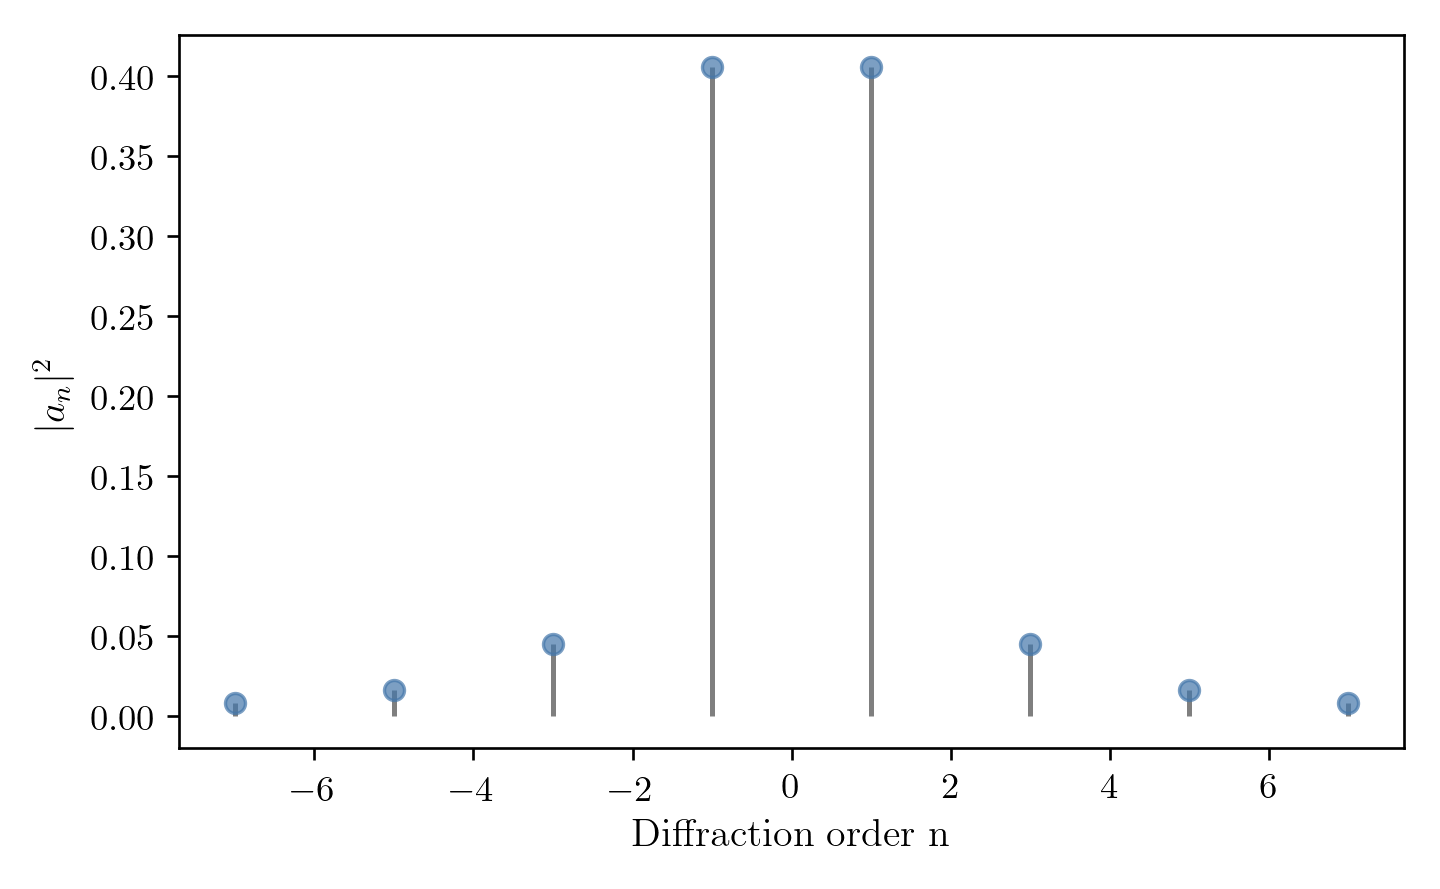
\includegraphics[width=0.8\textwidth]{figures/Two_source/a_n.png}
	\caption{Square complex modulus of the Fourier coefficients $a_n$ of the $0-\pi$ SWPG. The square complex modulus is proportional to the energy put into each diffraction order.  As can be seen from figure, the $\pm1$ orders have the most energy put into them at $4/\pi^2\approx41.1\%$ each.  All even orders have zero energy.}
	\label{fig:a_n}
\end{figure}

With these Fourier coefficients in hand, we can now calculate the field profile at the focus.  This is done by using equation \ref{eqn:field_at_focus},
\begin{equation}
\label{eqn:swpg_field_at_focus}
	\begin{aligned}
		\tilde{S}(\tilde{x}) &= \frac{i k A}{2\pi f}e^{ikf}e^{i\frac{k\tilde{x}^2}{2f}}\int_{-\infty}^{\infty}S(x,x_0)e^{-ikx\tilde{x}/f}\diff x\\
		\tilde{S}(\tilde{x}) &= \frac{i k A}{2\pi f}e^{ikf}e^{i\frac{k\tilde{x}^2}{2f}}\int_{-\infty}^{\infty} E(x) \sum_{n=-\infty}^{\infty}a_n(x_0)e^{-i\frac{2\pi nx}{d}} e^{-ikx\tilde{x}/f}\diff x\\
		\tilde{S}(\tilde{x}) &= \frac{i k A}{2\pi f}e^{ikf}e^{i\frac{k\tilde{x}^2}{2f}}\sum_{n=-\infty}^{\infty}a_n(x_0) \int_{-\infty}^{\infty} E(x) e^{-i\frac{2\pi x}{\lambda f}(\tilde{x} - n\frac{\lambda f}{d})}\diff x\\
		\tilde{S}(\tilde{x}) &= \sum_{n=-\infty}^{\infty} a_n(x_0) \tilde{E}(\tilde{x} - \tilde{x}_n)
	\end{aligned}
\end{equation}
where
\begin{equation}
	\tilde{E}(\tilde{x}) = \frac{i k A}{2\pi f}e^{ikf}e^{i\frac{k\tilde{x}^2}{2f}} \int_{-\infty}^{\infty}E(x)e^{-ikx\tilde{x}/f}\diff x,
\end{equation}
$x_n=n\lambda f/d$, $S(x,x_0)=E(x)P(x,x_0)$ is the field after the phase grating, and $A$ is a constant to account for the $y$ dimension in equation \ref{eqn:field_at_focus} which has been neglected for clarity in this discussion.  Substituting in equation \ref{eqn:swpg_fourier_coeff_a_n} into equation \ref{eqn:swpg_field_at_focus} yields
\begin{equation}
\label{eqn:swpg_field_at_focus_simple}
	\tilde{S}(\tilde{x}, x_0)=\sum_{n\neq 0}\mathrm{sinc}(\frac{n\pi}{2})\tilde{E}(\tilde{x}-\tilde{x}_n)e^{-in\frac{2\pi x_0}{d}}
\end{equation}
which is the field at the focal plane. From this equation, the role of the transverse offset $x_0$ immediately becomes clear.  It is used to control the relative phase between diffraction orders of the SWPG.  The phase difference between the two most populated orders, the $n=\pm 1$ orders, is given by
\begin{equation}
\label{eqn:phase_diff}
	\Delta\phi_{\pm 1}=2\bigg(\frac{2\pi x_0}{d}\bigg).
\end{equation}
Therefore, by controlling the offset of the SWPG we can control the relative phase between the two orders of interest over a range of $[0,4\pi]$, two full periods of the fundamental wavelength.  Additionally, one can begin to see from equation \ref{eqn:field_at_focus} that the intensity profile at the focal plane consists of copies of the focused input field at $x_n = n\lambda f/d$.  An example intensity profile at the focal plane is shown in figure \ref{fig:s^2}. In this figure the $\pm1$ orders are shown to be the most intense, and the phase is extracted for two different grating offset positions $x_0$.  This calculated by numerically propagating the beam profile and SWPG in figure \ref{fig:LP_inputs}.
\begin{figure}
	\centering
	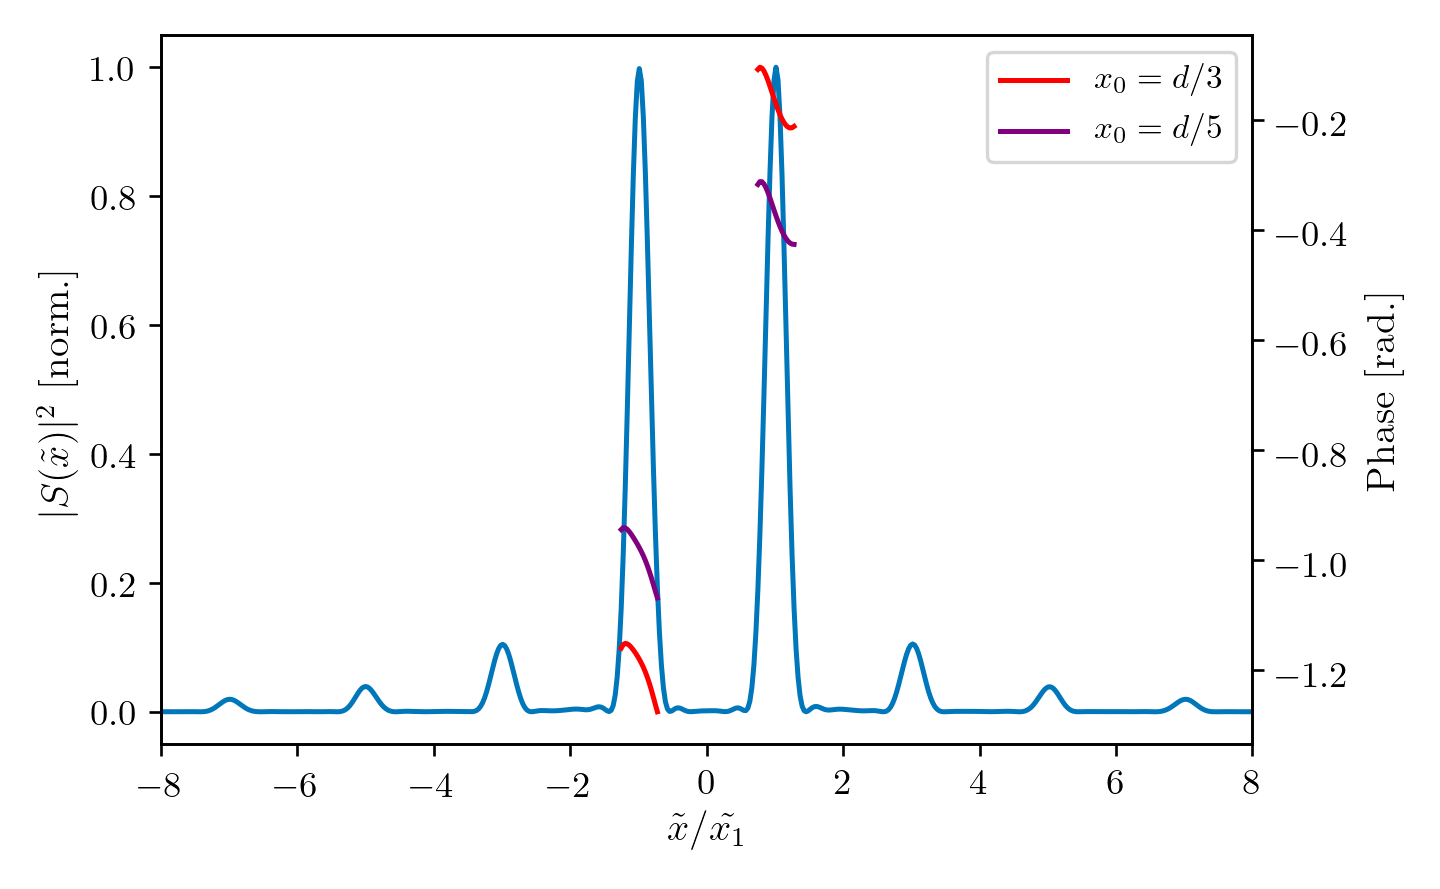
\includegraphics[width=0.8\textwidth]{figures/Two_source/intensity_and_phase.png}
	\caption{Intensity profile $S(\tilde{x})$ at the focal plane. Horizontal units are scaled by the spacing between orders, $\tilde{x_1}=\lambda f/d$.  Phase is also plotted for two different offset positions $x_0=d/3$ and $x_0=d/5$.  This demonstrates the ability of the SWPG to generate two sources and control the relative phase between them. Calculated by numerically propagating the beam profile and SWPG in figure \ref{fig:LP_inputs}.}
	\label{fig:s^2}
\end{figure}
\begin{figure}
	\centering
	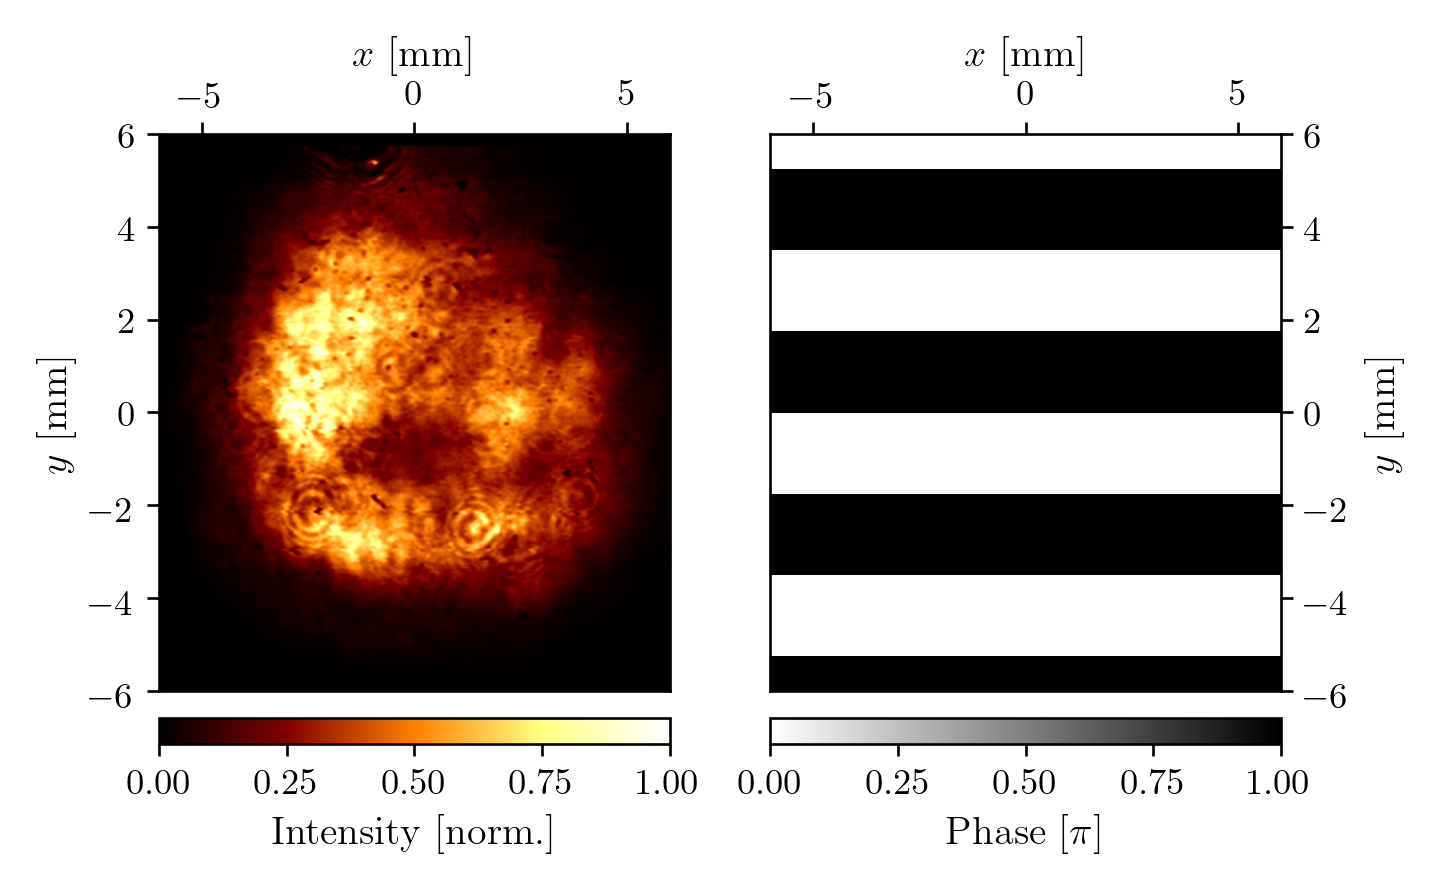
\includegraphics[width=0.9\textwidth]{figures/Two_source/LP_images.png}
	\caption{(a) Intensity profile of the input beam measured by a thermal camera. (b) Phase imparted by $0-\pi$ SWPG with a grating period of $d=$2.5 mm.}
	\label{fig:LP_inputs}
\end{figure}

So far, we have demonstrated that a binary $0-\pi$ SWPG can theoretically achieve our requirements of an efficient beam duplicator with phase control between the two duplicate beams.  However, all of the results shown above have been only considering the monochromatic case, and for the experiments of interest we will using a femtosecond IR pulse with bandwidth on the order of 50 nm.  This presents a challenge because the SWPG will be constructed by etching a fused-silica plate to have the desired phase step of $\pi$, and the inherent dispersion as the beam passes through the material means that the step will be $\pi$ for only one wavelength.  Thus, it is important to get a handle on how an imperfect non-$\pi$ phase step affects the properties of the SWPG.  To do this, we introduce a non-$\pi$ phase step into the above analysis by a parameter $\zeta$, such that the $0-\pi$ step becomes a $0-\zeta\pi$ step,
\begin{equation}
\label{eqn:zeta}
	\phi(x,x_0,\zeta)=\zeta \phi(x,x_0).
\end{equation}
Going back to \ref{eqn:a0_no_zeta}, we can calculate the zero-order term for $\zeta\neq1$,
\begin{equation}
\label{eqn:a_0_zeta}
	\begin{aligned}
	a_0(x_0,\zeta) &= \frac{1}{d}\int_{-\frac{d}{2}}^{\frac{d}{2}} e^{\zeta\phi(\tilde{x},x_0)}\diff\tilde{x}\\
	&= \frac{1}{d}\Bigg[\int_{-\frac{d}{2}}^{-\frac{d}{4}+x_0}e^{i\zeta\pi}\diff\tilde{x}
	+ \int_{-\frac{d}{4}+x_0}^{\frac{d}{4}+x_0} \diff\tilde{x}
	+ \int_{\frac{d}{4}+x_0}^{\frac{d}{2}} e^{i\zeta\pi}\diff\tilde{x} \Bigg]\\
	&=\frac{1}{d} \bigg[\frac{d}{2} + \frac{d}{2}e^{i\zeta\pi} \bigg] = \frac{e^{i\zeta\pi/2}}{2}\bigg[ e^{i\zeta\pi/2} 
	+ e^{-i\zeta\pi/2}\bigg]\\
	a_0 & = \cos\bigg(\frac{\pi}{2}\zeta\bigg)e^{i\zeta\pi/2}.
	\end{aligned}
\end{equation}
Previously, for $\zeta=1$ we found that the zeroth-order term was not populated by the SWPG ($a_0=0$), however from the above equation we can clearly see that the non-$\pi$ phase step has introduced a population in the zeroth-order.  The percent of the total input energy that is placed into the zeroth order is $\rvert a_0(\zeta)\rvert^2=\cos^2(\zeta\pi/2)$. Furthermore, from equation \ref{eqn:swpg_fourier_coeff_a_n} we can also calculate the other orders for $\zeta\neq1$,
\begin{equation}
\label{eqn:a_n_zeta}
	\begin{aligned}
	a_n(x_0,\zeta) &= \frac{1}{d}\int_{-\frac{d}{2}}^{\frac{d}{2}} e^{\zeta\phi(\tilde{x},x_0)}e^{-i n \frac{2\pi\tilde{x}}{d}}\diff\tilde{x}\\
	&= \frac{1}{d}\Bigg[\int_{-\frac{d}{2}}^{-\frac{d}{4}+x_0}e^{i\zeta\pi-i n \frac{2\pi\tilde{x}}{d}} \diff\tilde{x}
	+ \int_{-\frac{d}{4}+x_0}^{\frac{d}{4}+x_0}e^{-i n \frac{2\pi\tilde{x}}{d}} \diff\tilde{x}
	+ \int_{\frac{d}{4}+x_0}^{\frac{d}{2}} e^{i\zeta\pi-i n \frac{2\pi\tilde{x}}{d}}\diff\tilde{x} \Bigg]\\
	a_n(x_0, \zeta) & = \mathrm{sinc}\bigg(\frac{n\pi}{2}\bigg)\sin\bigg(\frac{\pi}{2}\zeta\bigg) e^{i\frac{\pi}{2} (\zeta - 1)} e^{-in\frac{2\pi x_0}{d}}\\
	a_n(x_0,\zeta) &= a_n(x_0)\sin\bigg(\frac{\pi}{2}\zeta\bigg)e^{i\frac{\pi}{2}(\zeta-1)}.
	\end{aligned}
\end{equation} 
From this equation, we can see that the non-$\pi$ phase step has not populated the even diffraction orders, but the odd orders have an overall phase shift and are reduced in amplitude by a factor of $\sin(\zeta\pi/2)$.  This should be expected because we saw from equation \ref{eqn:a_0_zeta} that the zeroth-order was populated by a fractional energy of $\rvert \cos(\zeta\pi/2)\rvert^2$.  Since this is a lossless system ($\sum_{n}\rvert a_n\rvert^2 = 1$), the energy that is populating the zeroth-order is coming from all of the odd orders that were populated. This redistribution of energy by $\zeta\neq1$ is shown in \ref{fig:a_n_zeta}.

\begin{figure}
	\centering
	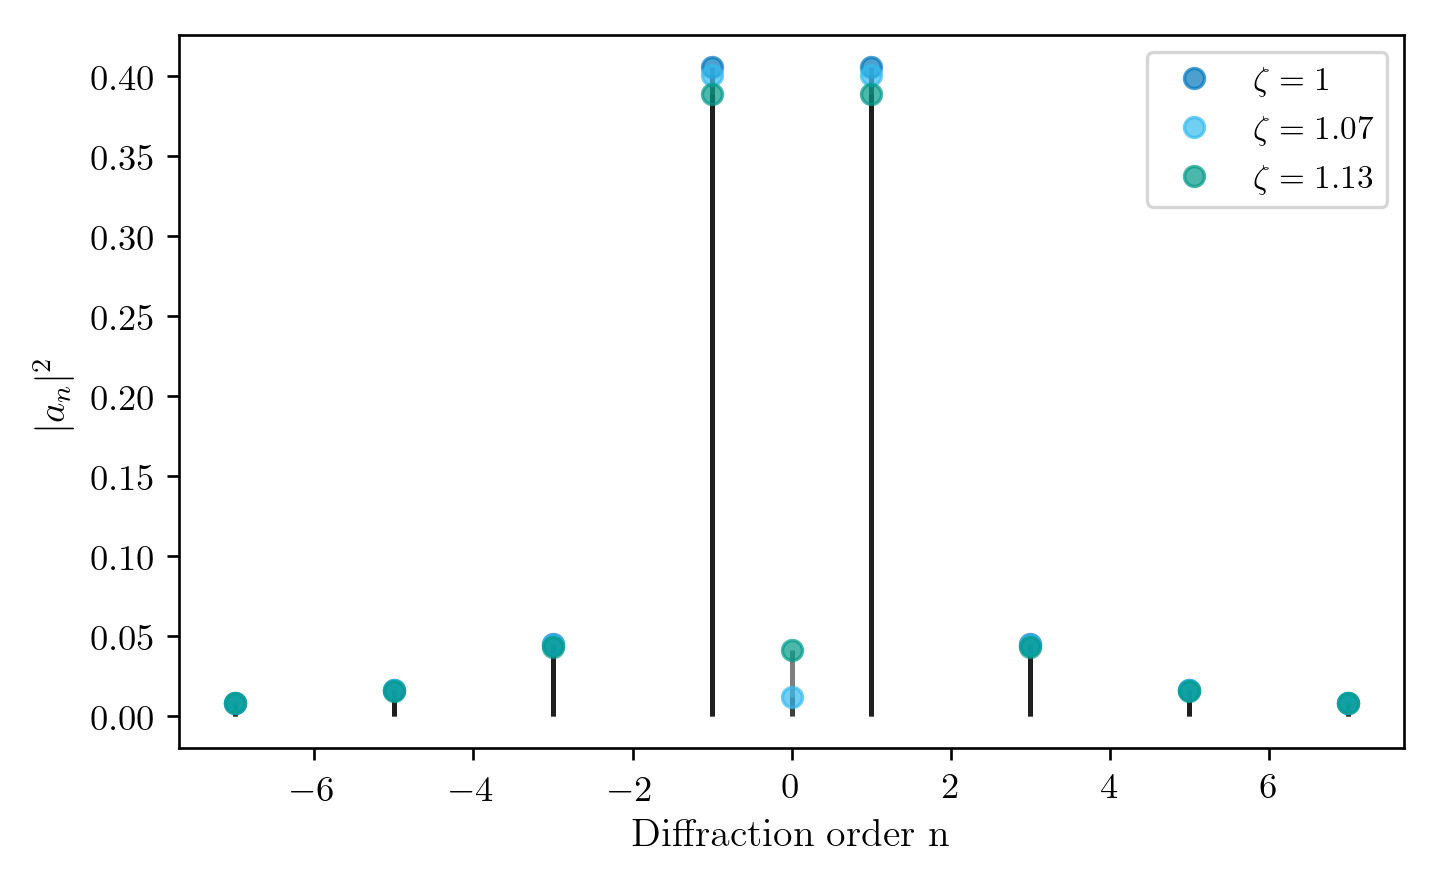
\includegraphics[width=0.8\textwidth]{figures/Two_source/a_n_zeta.png}
	\caption{Square complex modulus of the Fourier coefficients $a_n$ of the $0-\zeta\pi$ SWPG for several values of $\zeta$. The square complex modulus is proportional to the energy put into each diffraction order.  As can be seen from figure, the $\pm1$ orders have the most energy put into them even for $\zeta\neq 1$.  All non-zero even orders have zero energy.}
	\label{fig:a_n_zeta}
\end{figure}

From equations \ref{eqn:a_0_zeta} and \ref{eqn:a_n_zeta}, we now have a notion of how the SWPG is behaving across the bandwidth of our femtosecond pulses.  In particular, so long as $\zeta$ is close to 1, then the $\pm1$ orders are still the most intense, and as the grating offset $x_0$ is varied the phase difference between the $\pm1$ orders remains $\Delta\phi_{\pm1}=2\bigg(\frac{2\pi x_0}{d}\bigg)$ even though the overall spectral phase is modified by a factor of $e^{i\zeta\pi/2}$.  To set a scale for what $\zeta$ close to 1 means, consider the case when the zeroth-order is equal in amplitude to the the $\pm3$ orders, $\rvert a_0(x_0,\zeta)\rvert = \rvert a_{\pm3}(x_0,\zeta)\rvert$.  In this case, $\rvert \xi - 1\rvert=\rvert\frac{2}{\pi}\tan^{-1}(3\pi/2)-1\rvert\approx0.13$.  Therefore, it is reasonable to state the $0-\pi$ SWPG maintains its phase control duplication properties for $\rvert\zeta - 1\rvert<0.13$.

\subsection{Square-wave phase grating design for high-harmonic generation}
With the theory behind the SWPG well established, the specific grating parameters that were chosen with HHG in mind will be discussed in this section.  The laser source that will be considered is the output of a HE-TOPAS optical parametric amplifier produced by Light Conversion.  The TOPAS is pumped by a Spitfire ACE Ti:Sapphire system from Spectra-Physics.  The Spitfire ACE system is capable of producing  12 mJ, 60 fs (20 nm FWHM bandwidth) pulses at 1 kHz.  Using this system, the TOPAS is able to generate up to a combined 6 mJ of signal and idler. The signal wavelength range is from 1200 nm to 1600 nm, and within this range the TOPAS can output a nominally 70 fs pulse of up to 3 mJ with a tuneable central wavelength.  A design wavelength of 1350 nm was chosen for the SWPG because the TOPAS performance is optimal around this wavelength (see figure \ref{fig:TOPAS_output}).
\begin{figure}
	\centering
	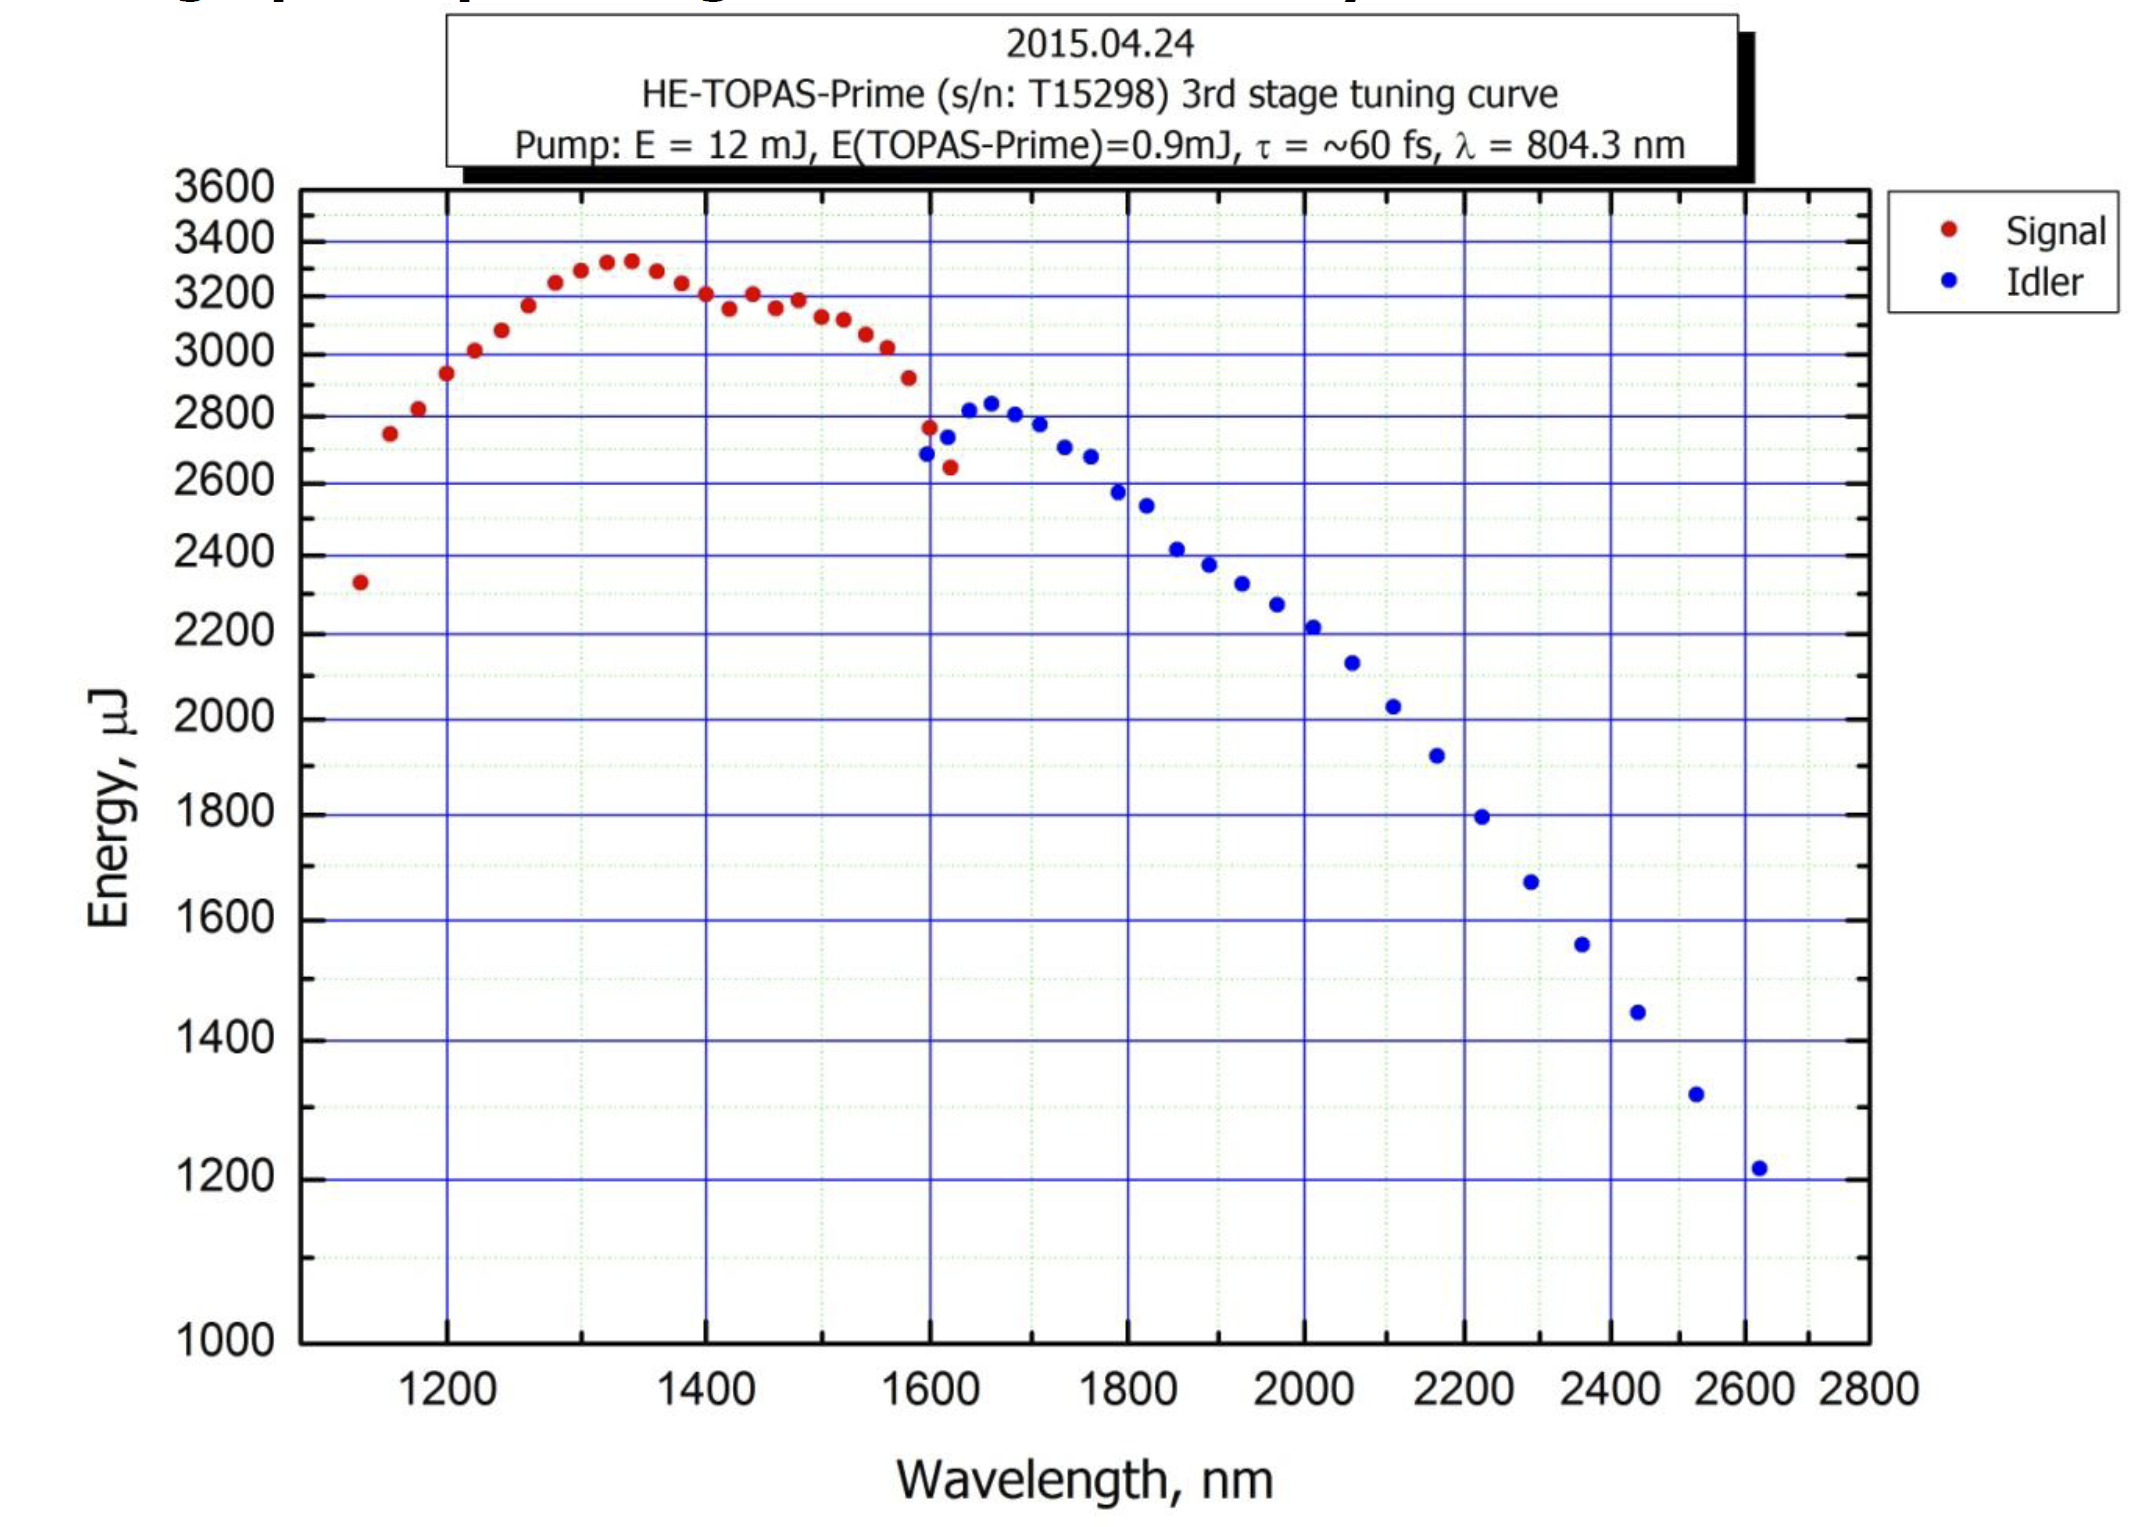
\includegraphics[width=0.7\textwidth]{figures/TOPAS/Topas_output.png}
	\caption{Pulse energy output of the TOPAS used in the experiments described within this chapter.  The optimal output energy of the TOPAS can be seen to be around 1350 nm.  This is the wavelength that was selected as the design wavelength for the SWPG.}
	\label{fig:TOPAS_output}
\end{figure}

Once the design wavelength for the phase grating is selected, then the physical size, $L$, of the step is determined by dispersion of the material selected from the relationship $\phi=\pi=2\pi n L/\lambda$.  For our phase gratings, Corning HPFS 7980 was used, and with this material $L\approx0.47\mu m$.  The refractive index and the corresponding $\zeta$ parameter is shown in figure \ref{fig:n_zeta}. The limitation that $\zeta=1$ for only the design wavelength can be relaxed somewhat by introducing a nonzero angle of incidence between the incoming beam and the SWPG to effectively increase the optical path length of the step.  If this angle is $\theta$, then the $\zeta$ parameter can be written as
\begin{equation}
\label{eqn:zeta_theta}
	\zeta(\lambda,\theta)=\sec\theta\bigg(  \frac{n(\lambda)\lambda_0}{\lambda n_0} \bigg)
\end{equation}
where $\lambda_0$ is the design wavelength and $n_0$ is the refractive index at the design wavelength.  This factor is shown in figure \ref{fig:n_zeta}.  From this figure, it is clear that even though the SWPG is designed for a specific wavelength it can be used over a broad range of wavelengths that are longer than the design wavelength. Of course, at higher angles of incidence propagation effects might become non-negligible, and those effects are neglected here. 
\begin{figure}
	\centering
	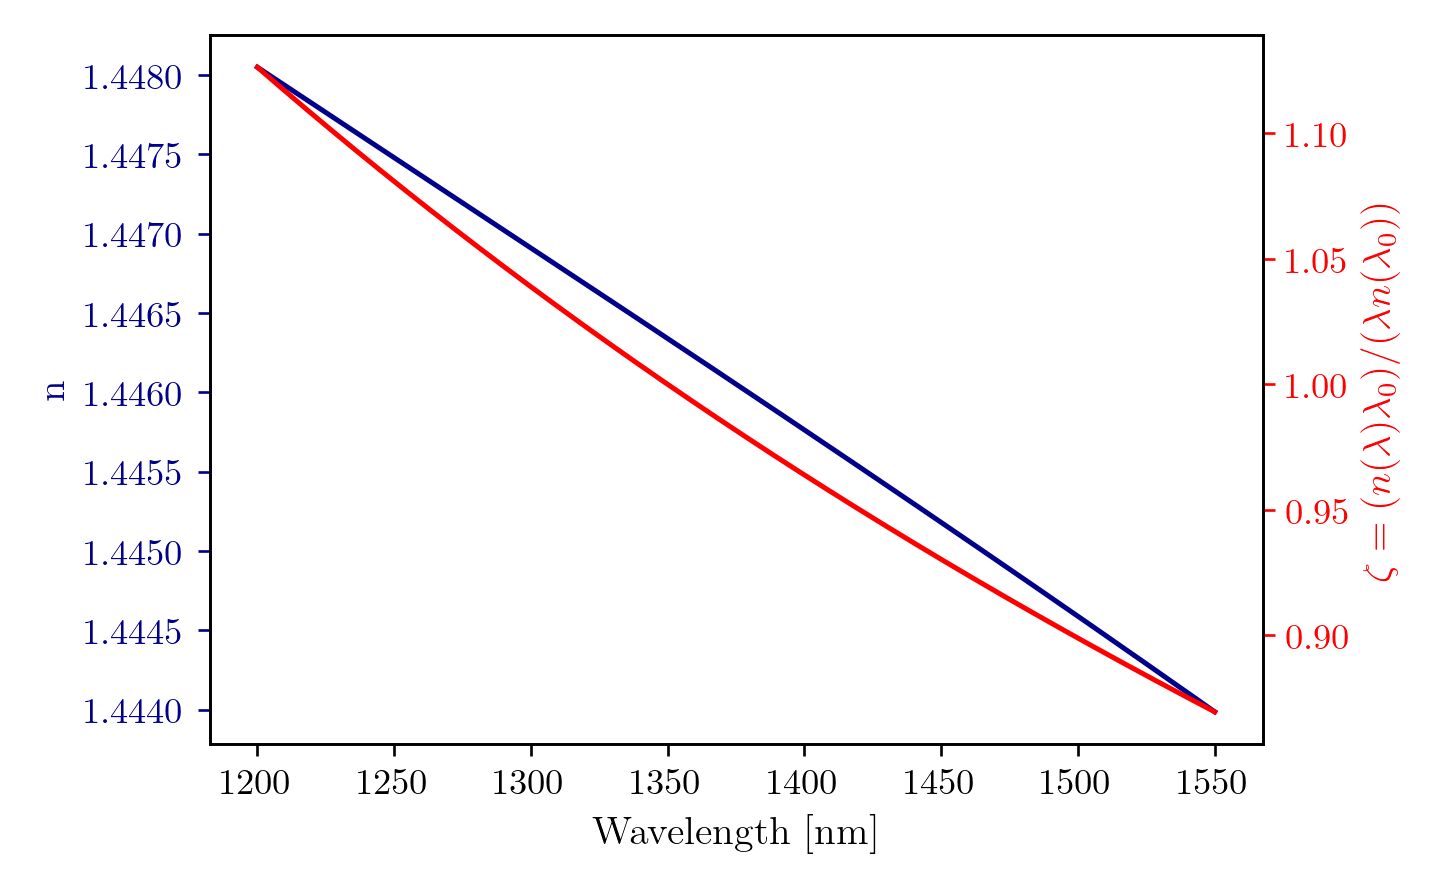
\includegraphics[width=0.75\textwidth]{figures/Two_source/n_zeta.png}
	\caption{Refractive index (blue curve and axis) and the $\zeta$ parameter (red curve and axis).  For a 70 nm bandwidth pulse centered at 1350 nm, $\zeta - 1$ varies from -0.026 to 0.027 assuming normal incidence.}
	\label{fig:n_zeta}
\end{figure}

\begin{figure}
	\centering
	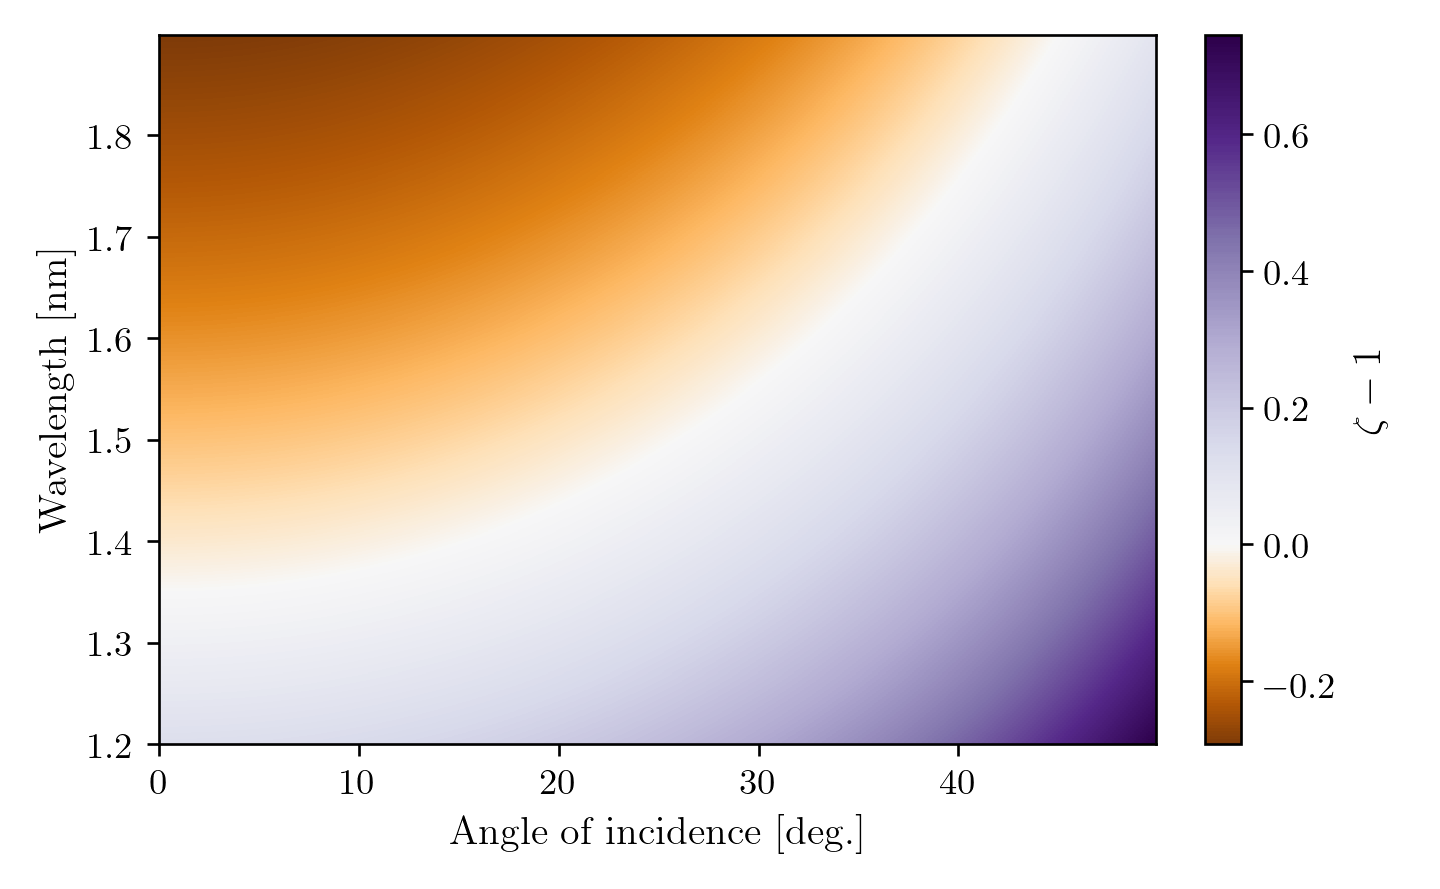
\includegraphics[width=0.8\textwidth]{figures/Two_source/zeta_theta.png}
	\caption{Non-$\pi$ phase step parameter $\zeta(\lambda,\theta)$ calculated for a range of relevant wavelengths and incident angles.  The ability to effectively tune the optical path length of the step enables the SWPG to be used for a much larger range of wavelengths that are longer than the initial design wavelength.}
	\label{fig:zeta_theta}
\end{figure}

The final remaining design parameter that must be considered is the choice of grating period. The choice of period is critical for the performance of the SWPG, and must be chosen with care.  To get insight into how to select the correct period, we will reintroduce the $\beta$ parameter from equation \ref{eqn:beta_parameter}.  For the specific situation we are considering, the $\beta$ parameter is
\begin{equation}
\label{eqn:beta_swpg}
	\begin{aligned}
		\beta &= \frac{2\pi \sigma D}{\lambda f} = \frac{2\pi\sigma\big(\frac{\lambda f}{d}\big)}{\lambda f}\\
		&= 2\pi\bigg(\frac{\sigma}{d}\bigg)
	\end{aligned}
\end{equation}
where $\sigma$ is the input beam radius and $D=\tilde{x}_1=\lambda f /d$ is that characteristic length scale at the focal plane because it represents the separation between the different diffraction orders in the focal plane.  The beam profile at the focus can be calculated for various parameters of $\beta$, and is shown in figure \ref{fig:intensity_vs_beta}.
\begin{figure}
	\centering
	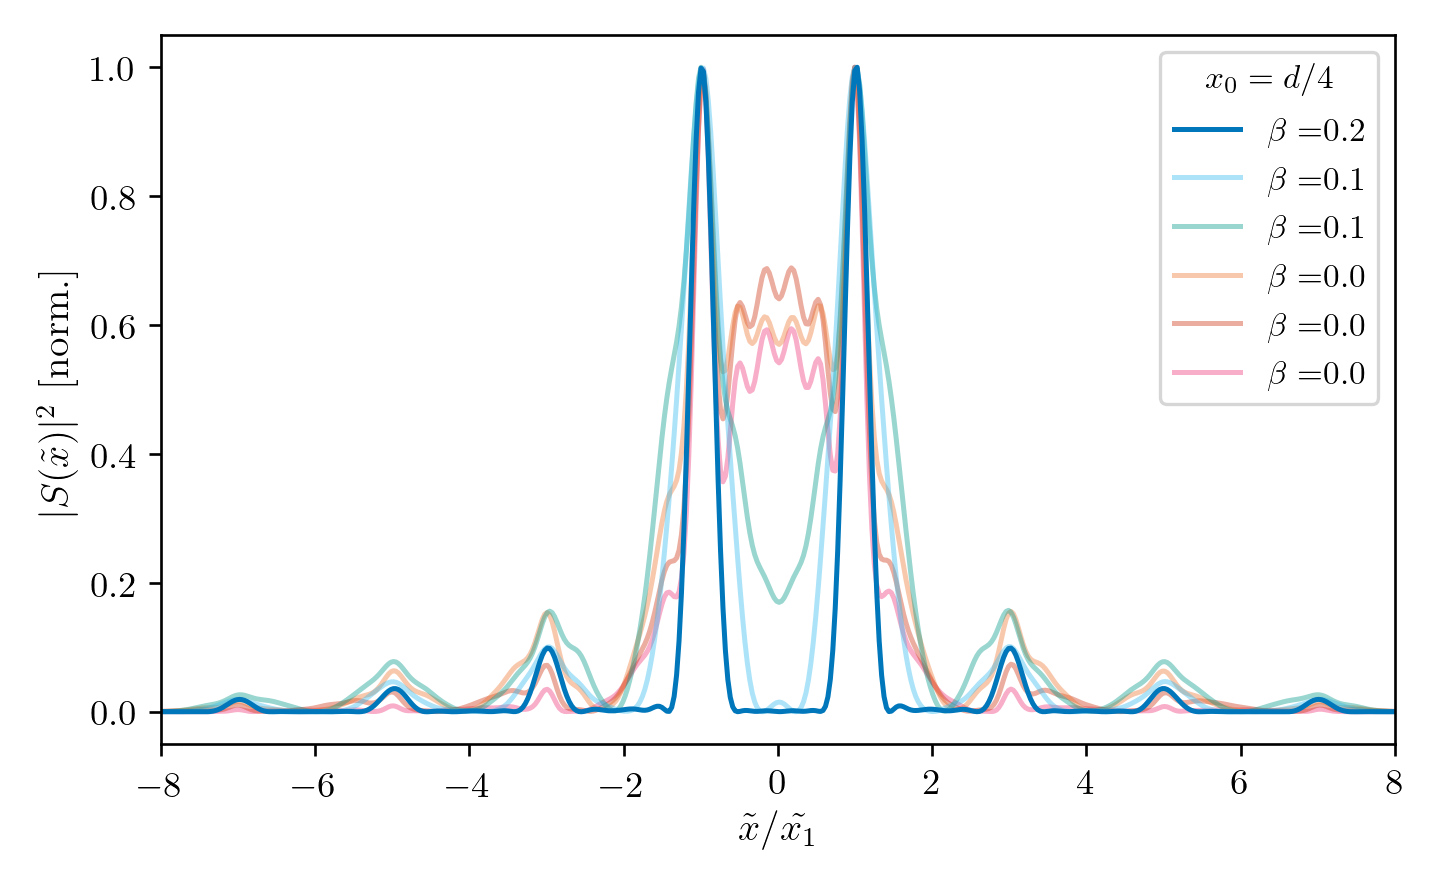
\includegraphics[width=0.8\textwidth]{figures/Two_source/focus_intensity_beta_sigma.png}
	\caption{Calculation of intensity at the focal plane of the SWPG for various parameters of $\beta$.  Calculation is done my numerically propagating the measured beam profile shown in \ref{fig:LP_inputs}.  $\beta$ is varied by adjusting the radius of the input beam profile.  As $\beta\rightarrow0$, one can see that the performance of the SWPG deteriorates and not longer produces well separated sources.}
	\label{fig:intensity_vs_beta}
\end{figure}
In the limit as $\beta\rightarrow0$, the condition $d\gg\sigma$ must hold, and this condition implies that the source separation is approaching the waist radius of each diffraction order $\tilde{\sigma}$.  Once the separation between orders becomes comparable to the waist ($\tilde{\sigma}\approx\tilde{x}_1$), then each diffraction order will strongly interfere with it's neighboring orders.  The effect of this interference is that our sources can no longer be thought of as independent beams, and as the grating offset $x_0$ is varied there will be a strong modulation of both the amplitude and phase of each of diffraction order.  This can be seen by using equation \ref{eqn:swpg_field_at_focus} to write the intensity at the focal plane
\begin{equation}
\label{eqn:intensity_modulation}
	\begin{aligned}
	\rvert\tilde{S}(\tilde{x},\phi_1)\rvert^2 &= \sum_{n=-\infty}^{\infty}\sum_{n'=-\infty}^{\infty} a_n \tilde{E}(\tilde{x} - \tilde{x}_n)e^{-in\phi_1}a_{n'} \tilde{E}(\tilde{x} - \tilde{x}_{n'})e^{-in'\phi_1}\\
	&= \sum_{q=-\infty}^{\infty}e^{-iq\phi_1}\sum_{n=-\infty}^{\infty} a_n\tilde{E}(\tilde{x}-\tilde{x}_n) a_{n-q}\tilde{E}(\tilde{x}-\tilde{x}_{n-q})\\
	&= \sum_{n=-\infty}^{\infty}\tilde{E}_{2n+1}^2(\tilde{x}) + 2\sum_{q=1}^{\infty}\cos(2q\phi_1) \sum_{n=-\infty}^{\infty}\tilde{E}_{2n+1}(\tilde{x})\tilde{E}_{2n-2q+1}(\tilde{x})
	\end{aligned}
\end{equation}
where $\tilde{E}_n(\tilde{x})=\rvert a_n\rvert\tilde{E}(\tilde{x} - \tilde{x}_n)$. The second term demonstrates that as the grating offset $x_0$ is varied, the intensity of a diffraction order $2n+1$ will be modulated by an oscillatory term $\cos(2q\phi_1)$.  The amplitude of this oscillation is determined by the overlap of the diffraction orders.  Thus, for a grating such that $d\gg\sigma$ the oscillations will be very large because the source separation will be comparable to the beam waist of each order.

While it has become clear that choosing a grating period such that $\sigma\gg d$ is the ideal case for the performance fo the SWPG as a beam duplicator, there is another consideration that must be made for our specific application.  In particular, we would like to generate high-harmonics from the $\pm1$ orders, and it order to do that we must send both sources through a gas medium generated by a gas jet in vacuum.  This becomes increasingly difficult to handle as the source separation becomes large because the nozzle diameter must also increase, and the throughput of the nozzle increases quadratically with the diameter \cite{scolesAtomicMolecularBeam1988}.  Since this needs to be done in vacuum, at a certain point the pumping requirements become untenable.  So, in light of these considerations, the grating periods that were chosen were 2.5 mm and 3.5 mm.  A schematic of the gratings are shown in figure \ref{fig:silios_sketch}.
\begin{figure}
	\centering
	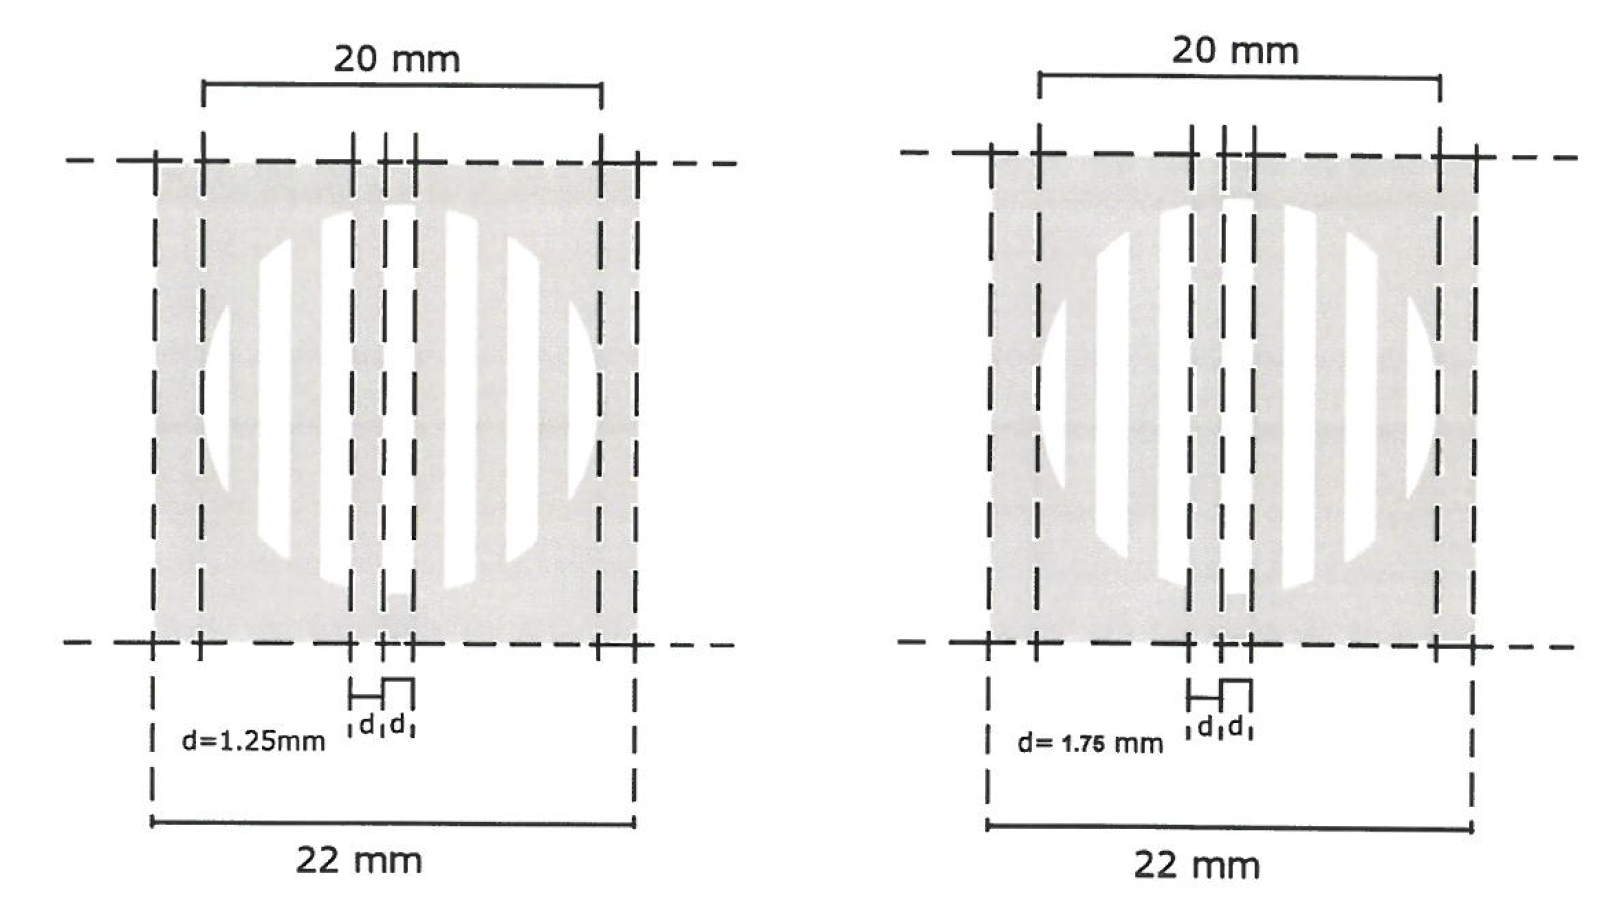
\includegraphics[width=0.6\textwidth]{figures/Two_source/silios_sketch.png}
	\caption{Schematic of the two SWPG which were purchased from Silios.  They are constructed by etching the phase step in Corning HPFS 7980 fused-silica.}
	\label{fig:silios_sketch}
\end{figure}
Using these gratings and a $f=400$ mm lens at 1450 nm, we are able to achieve a source separation of 331 $\mu m$ and 464 $\mu m$ for the grating periods $d=3.5$ mm and $d=2.5$ mm.  These parameters correspond to $\beta\approx7$ for the 3.5 mm grating and $\beta\approx10$ for the 2.5 mm grating for an input beam radius of $\sigma=4$ mm.

\section{Two-source high-harmonic generation}

To demonstrate that the $0-\pi$ SWPG can be used as a femtosecond beam duplicator with relative phase control, we will generate harmonics from the $\pm1$ diffraction orders.  This experiment will be performed in the transient-absorption beamline (TABLe), and a schematic is show in figure \ref{fig:schematic}.  A $0-\pi$ SWPG will be used to generate two intense lobes at the focal plane of a $\mathrm{CaF}_2$ plano-convex lens with a focal length of 400 mm.  A piezoelectric pulsed valve gas jet with a nozzle diameter of 500 $\mu m$ is placed near the focus to deliver a gas medium in which high-harmonics are generated.  The gas that will be used for generation will be argon.  An image of the two sources is shown in \ref{fig:piezo_jet}.  The laser which was used for this experiment is the output of an HE-TOPAS pumped by the Spitfire laser system.  We will be working with a central wavelength of 1435 nm and a pulse energy of 2 mJ.  The harmonics that are generated will pass through a 200 nm Al filter to filter out the fundamental. In the energy ranges that we will be generating harmonics, Al will transmit harmonics in the energy range of 20 - 72 eV.  After the metallic filter, the XUV will be pass through a mirror with a hole in it and it will be refocused by an ellipsoidal mirror with a demagnification of 3.  The XUV will then enter the spectrometer which consists of a Hitachi 1200 lines/mm variable line spaced (VLS) grating with a microchannel plate (MCP)/phosphor detector.  The output of the phosphor is imaged by an Andor Neo 5.5 camera.  The VLS grating focuses spectrally onto a flat-field, but in the transverse dimension it maintains the spatial profile. With this spectrometer we are able to simultaneously get spatial and spectral information about the incoming light.
\begin{figure}
	\centering
	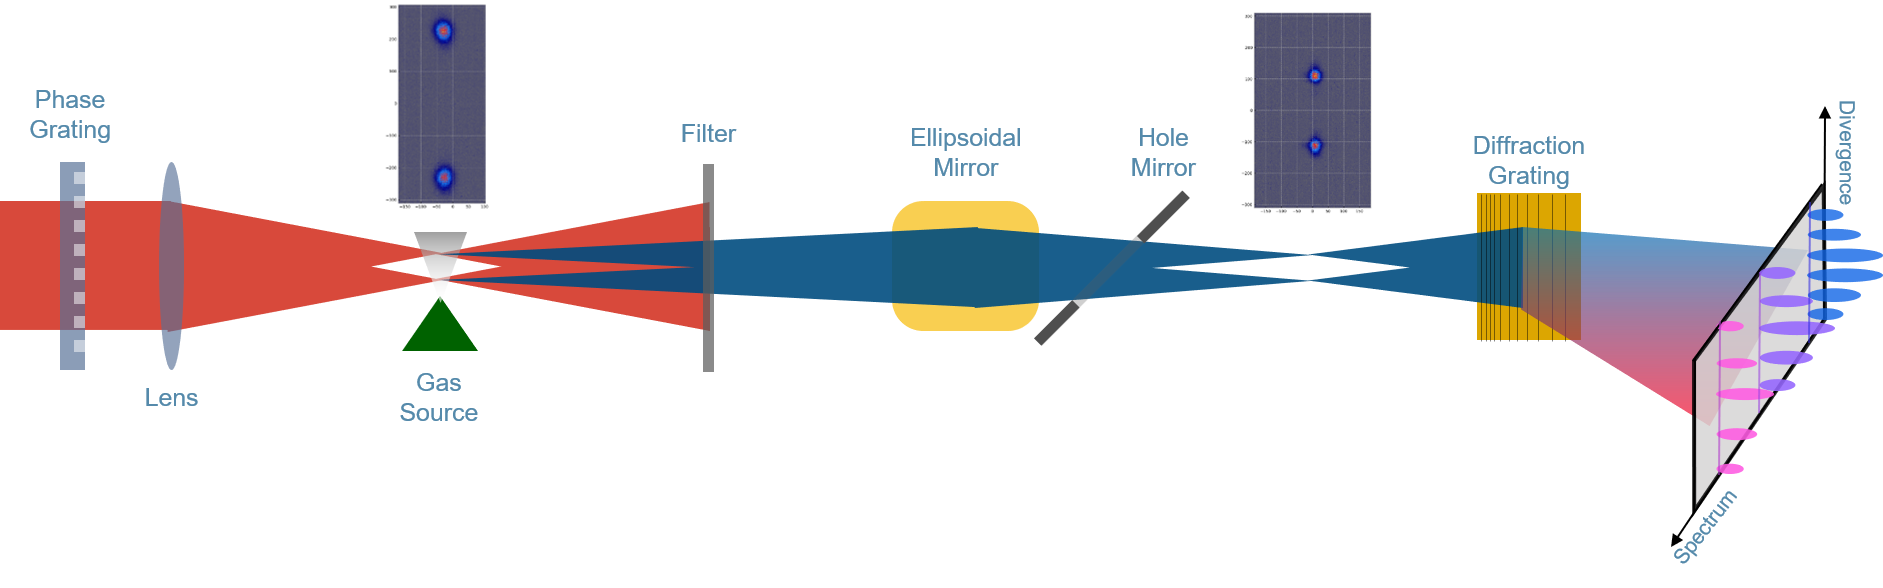
\includegraphics[width=0.8\textwidth]{figures/Two_source/schematic_table.png}
	\caption{Schematic of the two-source HHG experiment performed in the TABLe. A $0-\pi$ SWPG is used to generate two intense lobes at the focus of a lens.  These lobes will generate XUV beams which will interfere in the far-field.  An ellipsoidal mirror is used to refocus the XUV beams before going onto the spectrometer.}
	\label{fig:schematic}
\end{figure}
\begin{figure}
	\centering
	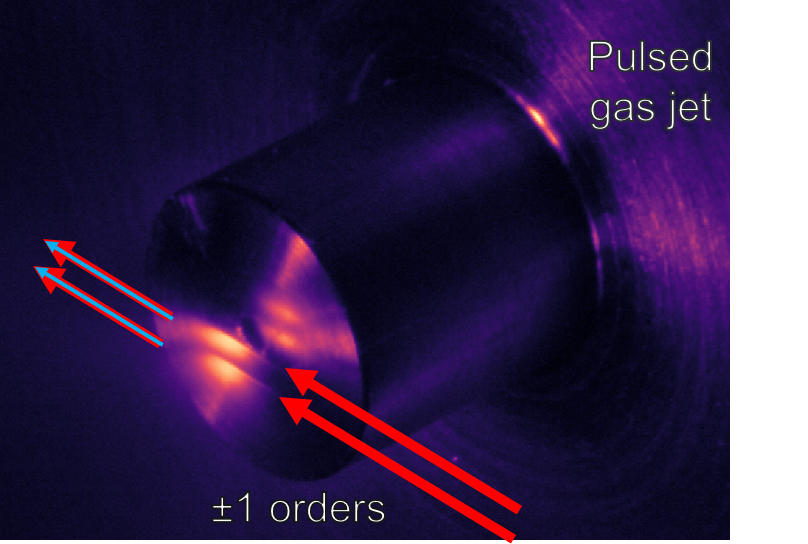
\includegraphics[width=0.6\textwidth]{figures/Two_source/pulse_jet_ts.png}
	\caption{False color image of the two sources from the SWPG driving ionization in a gas medium delivered by the piezo gas jet shown in the image.  Two sources follow the red arrows, and the XUV that is generated is shown by blue arrows.}
	\label{fig:piezo_jet}
\end{figure}

The harmonics that are generated from this setup are shown in figure \ref{fig:ref_img_pow_spec}. Along the spatial dimension (labeled sensor position in the figure), one can immediately see a fringe pattern.  These fringes are from the two sources that are generating harmonics.  The intuitive way to understand the spatial frequency of these fringes is by thinking of them in terms of a Young's double slit.  From this perspective, the wavelength dependence of the spatial frequencies present in the spatial profile of harmonic order $q$ is
\begin{equation}
	k_q=q\frac{2\pi \Delta x}{L \lambda}\propto q\hbar\omega
\end{equation} 
where $L$ is the distance from the two sources to the detector and $\Delta x$ is separation between the two sources.  This linear dependence of the spatial frequency on photon energy is clear seen in figure \ref{fig:ref_img_pow_spec}.
\begin{figure}
	\centering
	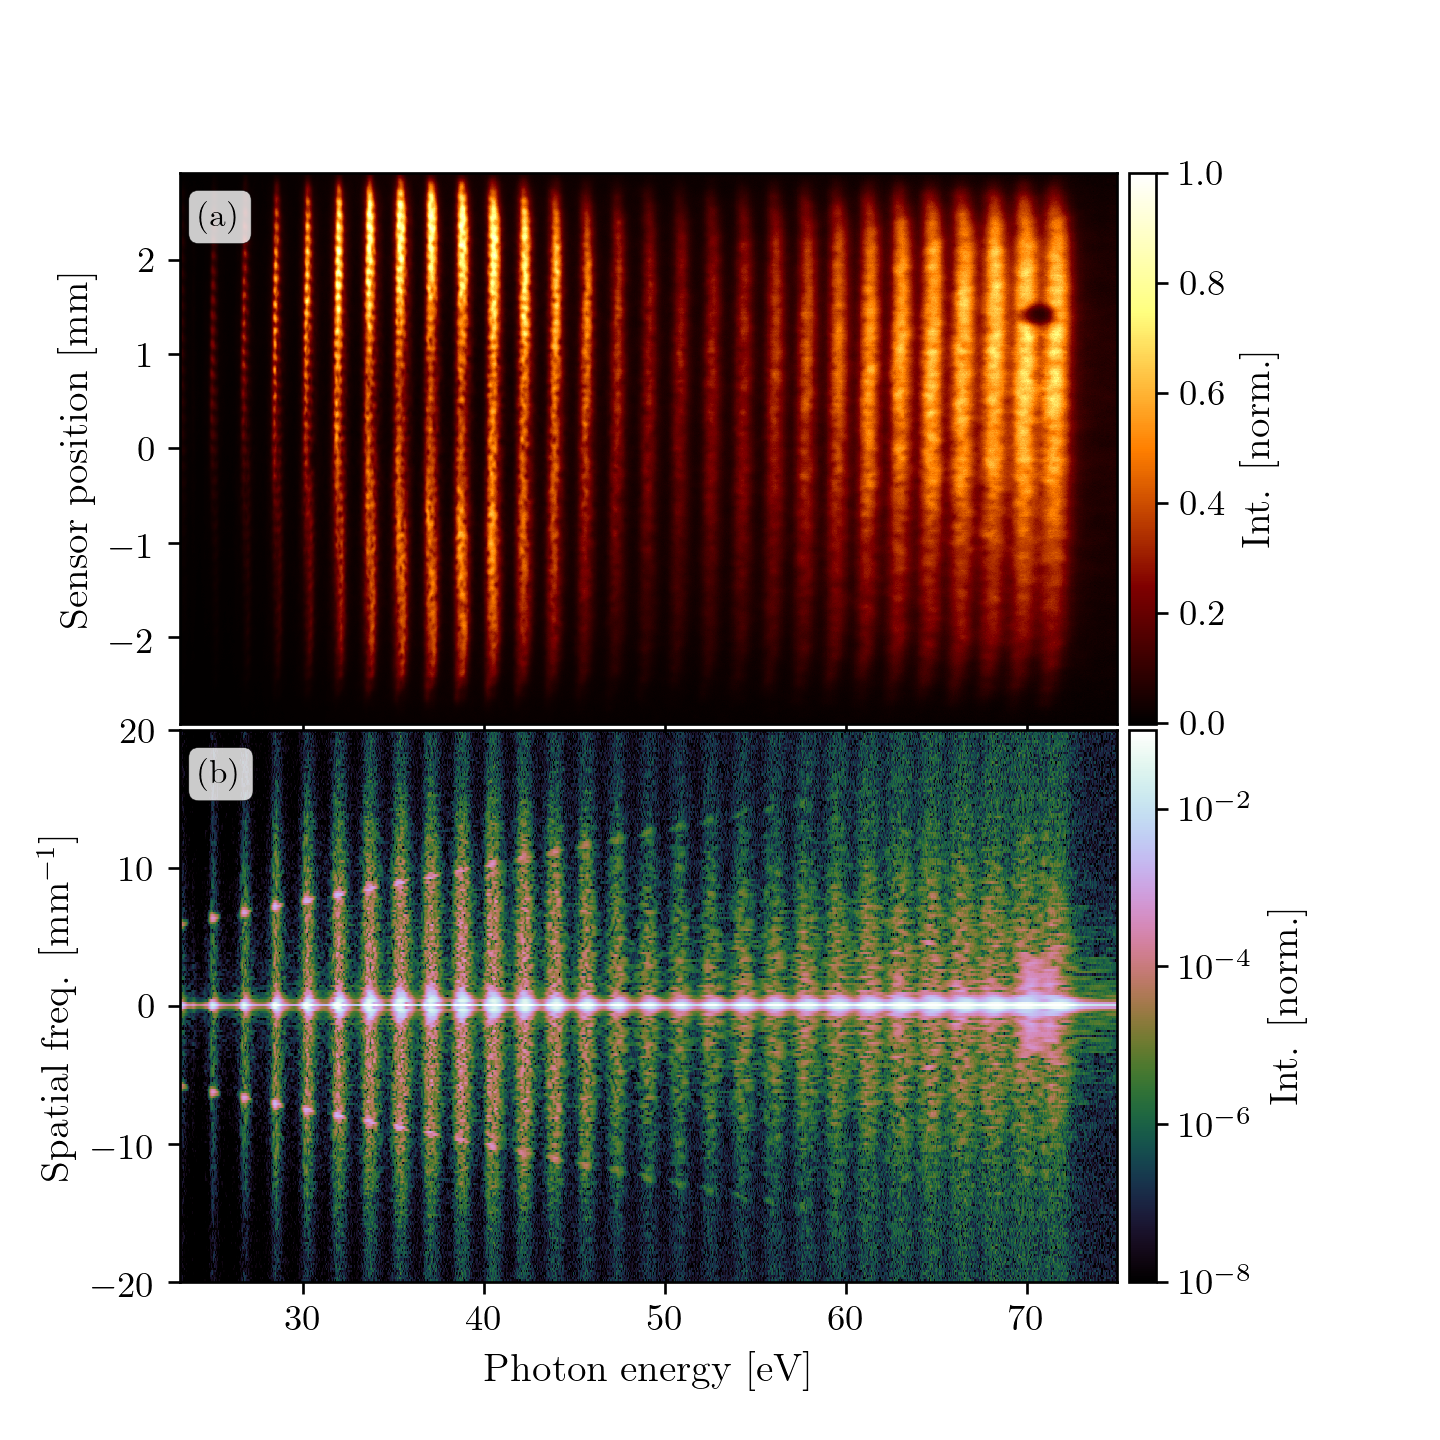
\includegraphics[width=1.0\textwidth]{figures/Two_source/ref_img_pow_spec.png}
	\caption{(a) Reference harmonic spectrum generated with a $0-\pi$ SWPG. The fringes along the sensor position dimension are due to interference between the two XUV sources that are generated.  The position of the fringe pattern is determined by the relative phase between the two sources.  This relative phase can be controlled by the SWPG. (b) Power spectrum of the Fourier transform of the above image along the sensor position dimension. Clear peaks can be seen corresponding to the spatial frequency for each harmonic order.  The linear dependence of the spatial frequency on photon energy is also seen.}
	\label{fig:ref_img_pow_spec}
\end{figure}

\begin{figure}
	\centering
	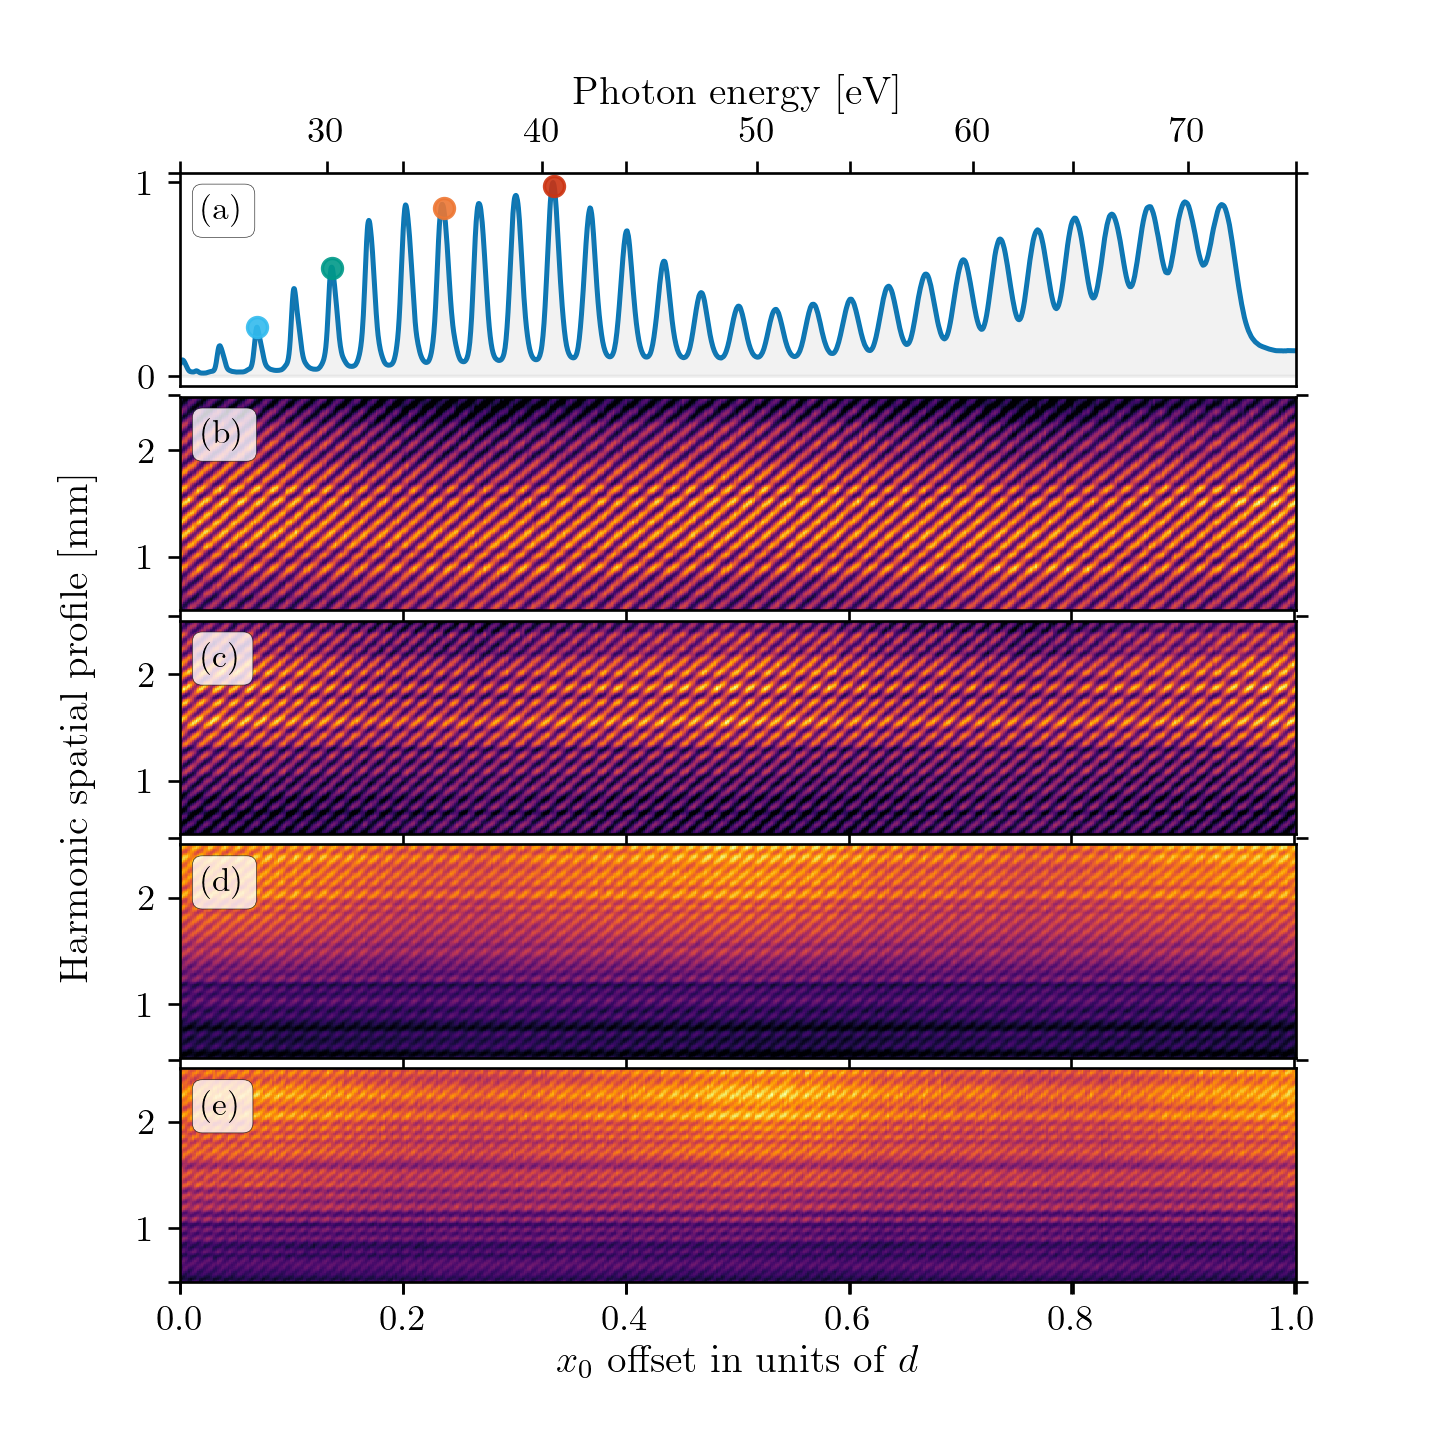
\includegraphics[width=1.0\textwidth]{figures/Two_source/harmonic_spatialgrams.png}
	\caption{(a) Reference harmonic spectrum with dots showing the harmonic orders whose spatialgrams are plotted below. (b)-(e) Spatialgrams for harmonic orders 29, 33, 39, and 45.  Tilted fringe pattern shows fringe shift due to phase shift induced by translating the phase grating. Modulations with a period od $d/2$ arise because of interference between the two generating sources.}
	\label{fig:harmonic_spatialgrams}
\end{figure}

The position of the fringe pattern in the spatial profile of the harmonics is determined by the relative phase between the two HHG sources.  Therefore, any phase shift between the two sources will be imprinted upon the spatial profile of the harmonics as a fringe shift.  We will utilize this sensitivity to demonstrate the capabilities of the SWPG.  If we generate harmonics from the $\pm1$ orders of the SWPG, then as the grating offset $x_0$ is varied we would expect the fringe pattern for harmonic order $q$ to shift by a factor of $q$ multiplied by the phase shift between the two IR sources. Thus, for a translation of the grating by $\Delta x_0$ the $q$-th harmonic fringe pattern will shift by $4q\pi\Delta x_0/d$.  If the grating is scanned through it's full period of $d$, then the phase difference between the two harmonic beams of order $q$ will span a range of phases up to $4q\pi$.  Due to the high  non-linearity of HHG, this technique is very sensitive to small shifts in phase between the two beams, and it is precisely this sensitivity that will be leveraged in later experiments to extract more information in transient absorption experiments.  It is important to be clear that we are not looking to measure the absolute phase difference between the two sources.  Instead, we are primarily interested in our ability to measure a very small phase difference between the two sources introduced by the SWPG.

The measured effect of translating the grating is shown in figure \ref{fig:harmonic_spatialgrams}. Four harmonics orders have been selected and their spatial profile have been plotted versus grating offset position $x_0$.  These types of figures will be referred to as a spatialgram. Each spatialgram exhibits a tilted fringe pattern that corresponds to the fringe shift induced by a phase shift between the two XUV sources.  As expected, the higher order harmonics have a higher frequency fringe pattern because of their shorter wavelength  If one counts the number of fringes over the full grating period scan, then one would find $2q$ fringes for harmonic order $q$. This provides a direct measure of the harmonic order $q$ and is used in a calibration scheme for the spectrometer (see chapter on calibration).  The ability to measure the harmonic order $q$ from the spatialgram verifies that the SWPG is able to control the phase difference between the two IR sources with a precision of a few mrad.

An additional feature of the spatialgrams in figure \ref{fig:harmonic_spatialgrams} is a slower modulation that has a period of $d/2$.  This effect is present for all harmonic orders, and appears in a very similar way.  This slower modulation is due to the interference between the two IR sources that were introduced in equation \ref{eqn:intensity_modulation}.  The modulations with a period of $d/2$ is due to interference between the $\pm1$ and $\mp1$ diffraction orders.  There is also a modulation with a period of $d$ that is present in the spatialgrams.  This modulation is due to interference between the 0th order and the $\pm1$ orders.  In general, the frequency of the modulations is related to the separation between the diffraction orders that are interfering.  These modulations are a limiting factor in using the phase grating for Fourier transform spectroscopy in the XUV.

Another interesting result from these measurements is that the symmetry of the attosecond pulse train (APT) that is generated can be observed because we are, in effect, measuring the interferometric autocorrelation of the XUV that is generated \cite{nabekawaInterferometryAttosecondPulse2013, nabekawaInterferometricAutocorrelationAttosecond2008, mengInterferometricTimeDelay2016, kovacevExtremeUltravioletFourierTransform2005}.  This is done either by looking at the zeroth-order diffraction off the VLS grating, or by integrating spectrally and looking at the combined spatial profile versus the grating offset.  The later technique is used to generate figures \ref{fig:full_spatialgram} and \ref{fig:full_spatialgram_w2w}.  In figure \ref{fig:full_spatialgram}, the pulses that make up the APT can be clearly seen.  Since the phase grating is limited to a scan range of $4\pi$ between the two IR sources, we would expect to see only four pulses (one per half-cycle), and this is exactly what is observed.  This can also be done in the case where the harmonics are generated using a two-color field consisting of the fundamental wavelength and it's second harmonic.  In this instance, the symmetry of the field is broken, and one should expect to see an attosecond pulse once per cycle of the fundamental \cite{kimHighlyEfficientHighHarmonic2005, dudovichSubcycleSpatialMapping2009, dudovichMeasuringControllingBirth2006}.  That exact case is shown in figure \ref{fig:full_spatialgram_w2w}.  In principle, by Fourier transforming these traces, one should be able to recover the harmonic spectrum with a spectral resolution of $\omega/2$.
\begin{figure}
	\centering
	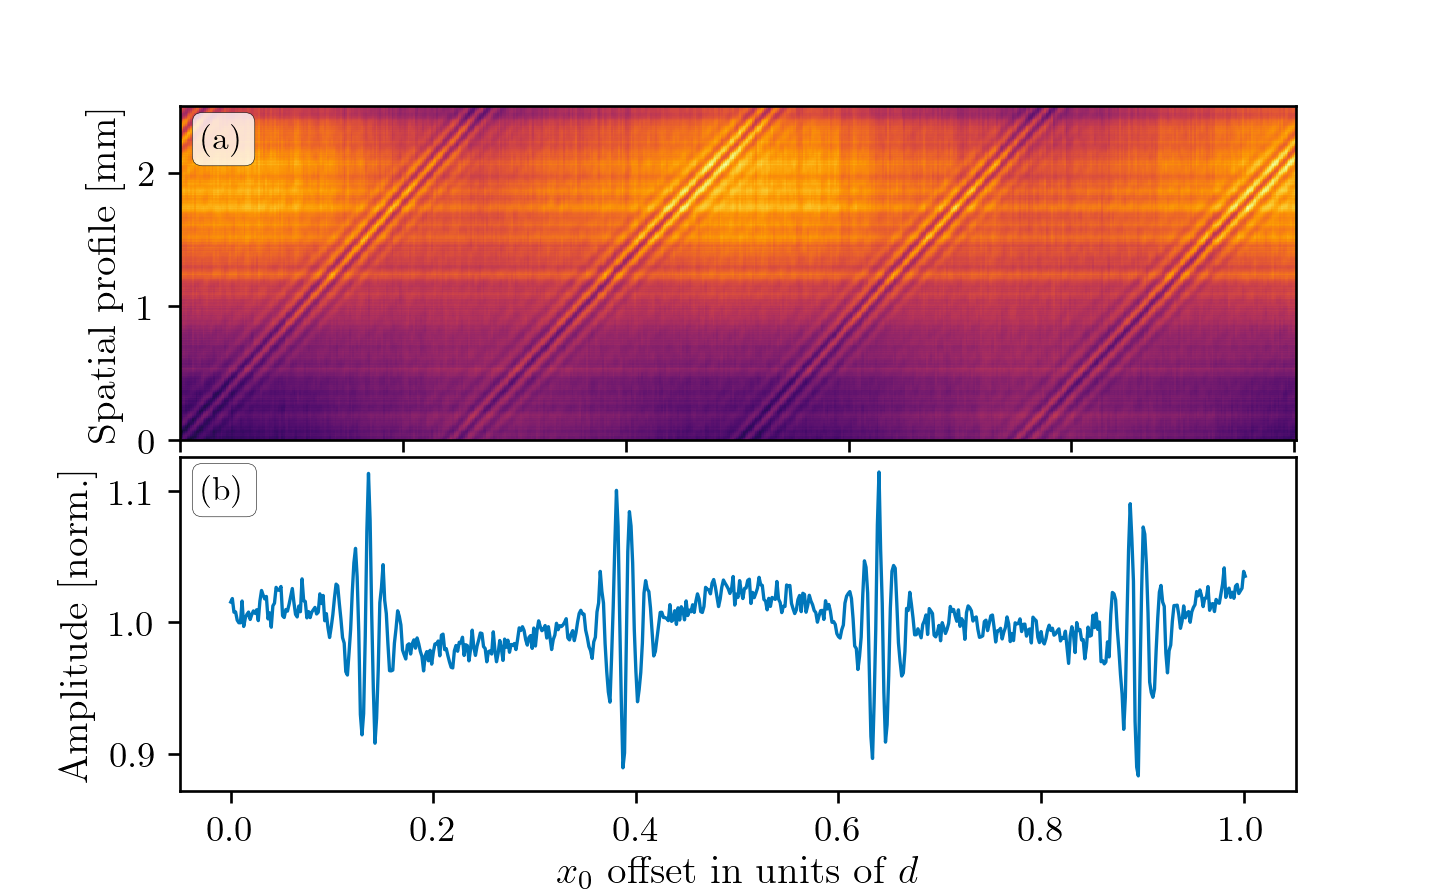
\includegraphics[width=1.0\textwidth]{figures/Two_source/full_spatialgram.png}
	\caption{(a) Spatialgram of all harmonic orders combined. Diagonal stripes show the attosecond pulses that make up the APT. (b) Lineout from the full spatialgram.  }
	\label{fig:full_spatialgram}
\end{figure}
\begin{figure}
	\centering
	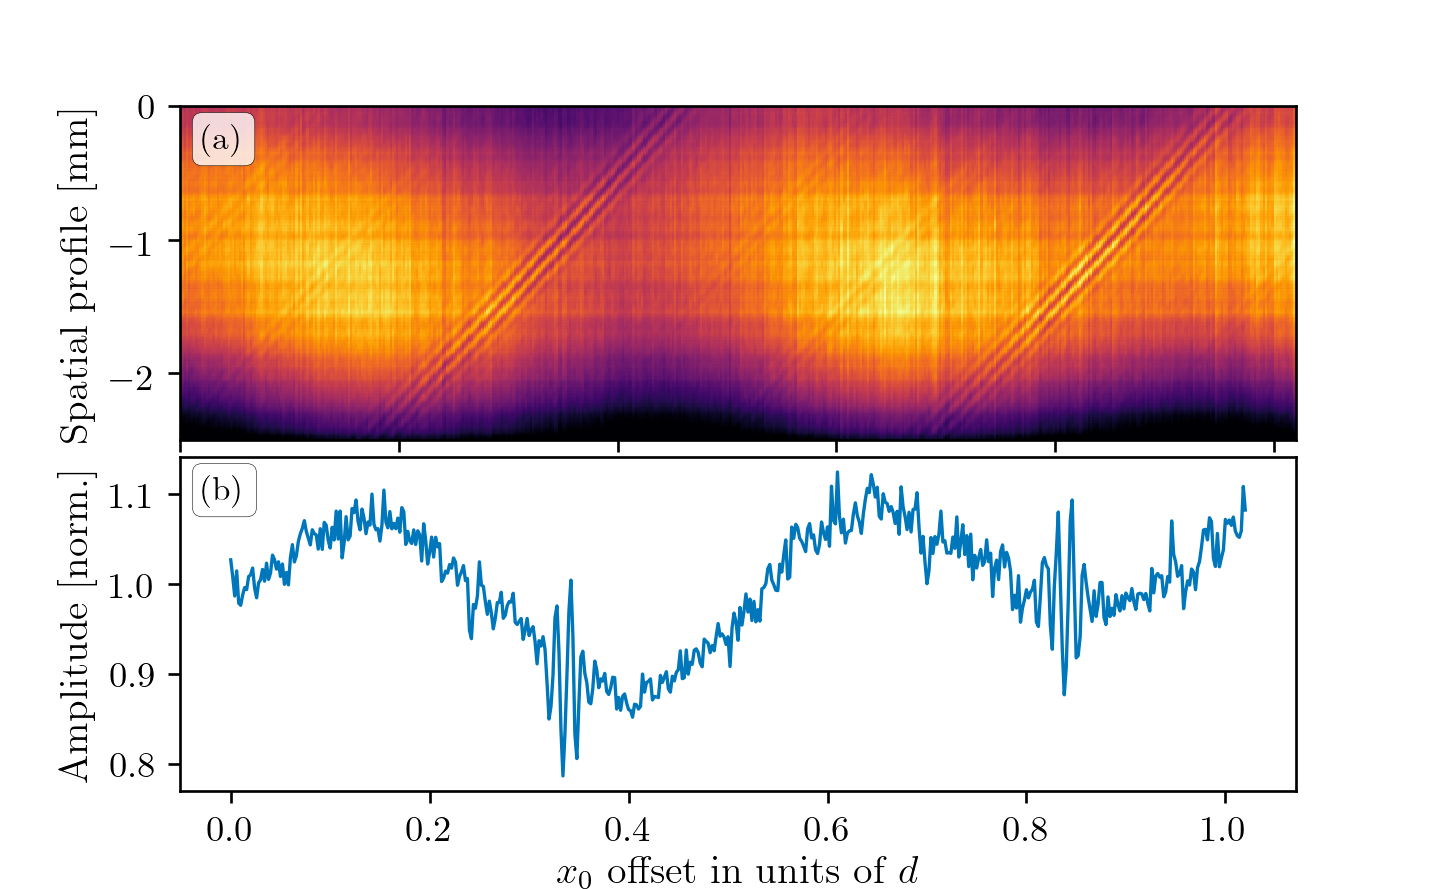
\includegraphics[width=1.0\textwidth]{figures/Two_source/full_spatialgram_w2w.png}
	\caption{(a) Spatialgram of all harmonic orders combined. Diagonal stripes show the attosecond pulses that make up the APT. A second harmonic field was added to break the symmetry and generate even harmonics. (b) Lineout from the full spatialgram.  Only two attosecond bursts are seen, which is expected from the asymmetric two-color generation field.  The increased modulation with a period $d/2$ is due to the stronger interference between the two sources.}
	\label{fig:full_spatialgram_w2w}
\end{figure}

\section{Conclusion}
In this chapter, the general concept of laser beam shaping was introduced, and the methods therein were applied to the specific problem of generating duplicates of a femtosecond IR pulse with precise control over their relative phase. The diffractive optical element that was shown to meet these demands is a $0-\pi$ square-wave phase grating (SWPG).  It's properties were discussed, and the final design parameters were chosen to optimize the SWPG for high-harmonic generation.  The properties of the SWPG were demonstrated by  generating high-harmonics and observing their corresponds fringe shifts.  This experiment has also demonstrated the ability measure small phase shifts between the two relative phase locked XUV beams.  This property will be leveraged in experiments described in the following chapters.
